

%%=============================================================================
%% Handleiding
%%=============================================================================

\chapter{Handleiding}
\label{ch:handleiding}

Dit hoofdstuk beschrijft hoe men het best te werk kan gaan voor het opzetten van een \textit{eenvoudig, kleinschalig blockchain-gebaseerd stemsysteem}. Het doel is om een praktische en complete handleiding te vormen, hoofdzakelijk bedoeld voor ontwikkelaars die niet vertrouwd zijn met het ontwikkelen van Ethereum DApps, noch met het ontwikkelen van cryptografische stemsystemen. 

Gezien de vrij technische aard van deze handleiding, wordt er verondersteld dat de lezer op zijn minst een algemene voorkennis van programmeren heeft en enigszins vertrouwd is met \textit{Javascript}. Kennis van de taal \textit{Solidity} wordt niet verondersteld. Tenslotte wordt verondersteld dat de lezer over een basiskennis Engels beschikt, daar de volledige codebasis in die taal geschreven is. 

De  verschillende implementatiekeuzes die hier worden gemaakt, gebeuren op basis van verschillende concepten en technieken die werden toegelicht in hoofdstuk \ref{ch:stand-van-zaken}. Zo wordt er bijvoorbeeld gekozen voor het Ethereum-platform als ontwikkelomgeving op basis van sectie \ref{sec:ethereum-en-smart-contracts} en wordt de veiligheid vergeleken met die van het `state-of-the-art' zelftellende OVNP \autocite{McCorry2017} uit sectie \ref{sec:OVNP}.

Dit hoofdstuk vormt de \textit{proof-of-concept} van deze scriptie, we trachten hier antwoord te bieden op een deel van de onderzoeksvragen van deze scriptie, met name: 
\begin{itemize}
	\item \textit{Welke tools heeft men nodig om een blockchain-gebaseerd stemsysteem op te zetten en wat zijn de voor- en nadelen hiervan?}
	\item \textit{Is een blockchain-gebaseerd stemsysteem opzetten haalbaar in de praktijk?} 
\end{itemize}

\section{Benodigdheden}
\label{sec:benodigdheden}
	De volgende zaken dienen geïnstalleerd te worden voor men van start kan gaan met het implementeren van een gedecentraliseerde Ethereum-blockchain applicatie:
	\begin{itemize}
		\item{Node.js}
		\item{npm}
		\item{Truffle}
		\item{Ganache}
		\item{Metamask}
	\end{itemize}
	Daarnaast heeft men ook nodig:
	\begin{itemize}
		\item{Een IDE code-editor naar keuze met syntax-ondersteuning voor Solidity}
		\item{Google Chrome}
	\end{itemize}
	\subsection{Node en npm}
	Node.js is een populaire runtime-omgeving waarmee Javascript op ieder platform uitgevoerd kan worden, zonder dat daarvoor een browser nodig is. Npm is een pakketbeheerder voor Javascript-code. Npm zit standaard in Node.js en is `s werelds grootste softwareregister. Open source-ontwikkelaars wereldwijd gebruiken het om pakketten te delen, veel organisaties gebruiken npm om ook hun privéontwikkeling te beheren (\ref{fig:nodejs}).\footnote{Verkregen en vertaald van https://docs.npmjs.com/about-npm/}
	
	Eenmaal node\footnote{node met npm is verkrijgbaar via https://nodejs.org} en npm\footnote{npm is ook apart verkrijgbaar via https://www.npmjs.com/get-npm} geïnstalleerd zijn, verifieert men de installatie via het console-commando: 
	\lstset{language=bash}
	\begin{lstlisting}[numbers=none]
	> node -v
	\end{lstlisting}Bij correcte installatie geeft dit de huidige node-versie terug, bijvoorbeeld \textit{v10.15.1}. 
	
	\begin{figure}
		
\includegraphics[width=\linewidth/2]{img/nodejs.png}
		
\includegraphics[width=\linewidth/2]{img/npm.png}
		\caption{De Node.js en npm logo's}
		\label{fig:nodejs}
	\end{figure}
	
	\subsection{Truffle}
	Truffle is een ontwikkelomgeving, testframework en asset pipline, gericht op het versoepelen van het Ethereum-ontwikkelproces. Het bevat ook verschillende code-templates die als basis kunnen worden gebruikt om gedecentraliseerde applicaties te ontwikkelen.
	
	Truffle kan eenvoudig geïnstalleerd worden via npm (mits dit voorgeïnstalleerd is) met het console-commando:
	 \lstset{language=bash}
	\begin{lstlisting}[numbers=none]
	> npm install truffle
	\end{lstlisting}
	\subsection{Ganache}
	Ganache\footnote{Ganache is verkrijgbaar via https://www.trufflesuite.com/ganache} is een applicatie die ontwikkelaars in staat stelt om een private Ethereum-blockchain op te zetten. We gebruiken deze blockchain gedurende de volledige ontwikkelperiode. Op deze manier kan men kosteloos smart contracts ontwikkelen en testen, als men direct op de Ethereum-hoofdketen ontwikkelt, is er immers aan iedere transactie een kost verbonden. 
	
	Ganache biedt ons  niet enkel een lokale blockchain, maar ook 10 Ethereum accounts om te gebruiken tijdens het ontwikkelen. Deze accounts hebben adressen die corresponderen met adressen op de lokale Ethereum-blockchain. Elke account is vooraf geladen met 100 nep-ether.
	
	Figuur \ref{fig:ganache-blockchain}: Eenmaal Ganache geïnstalleerd is, open we de applicatie. Door het kiezen van de optie \textit{quickstart} zetten we onmiddellijk een lokale blockchain op. 
	
	\begin{figure}
		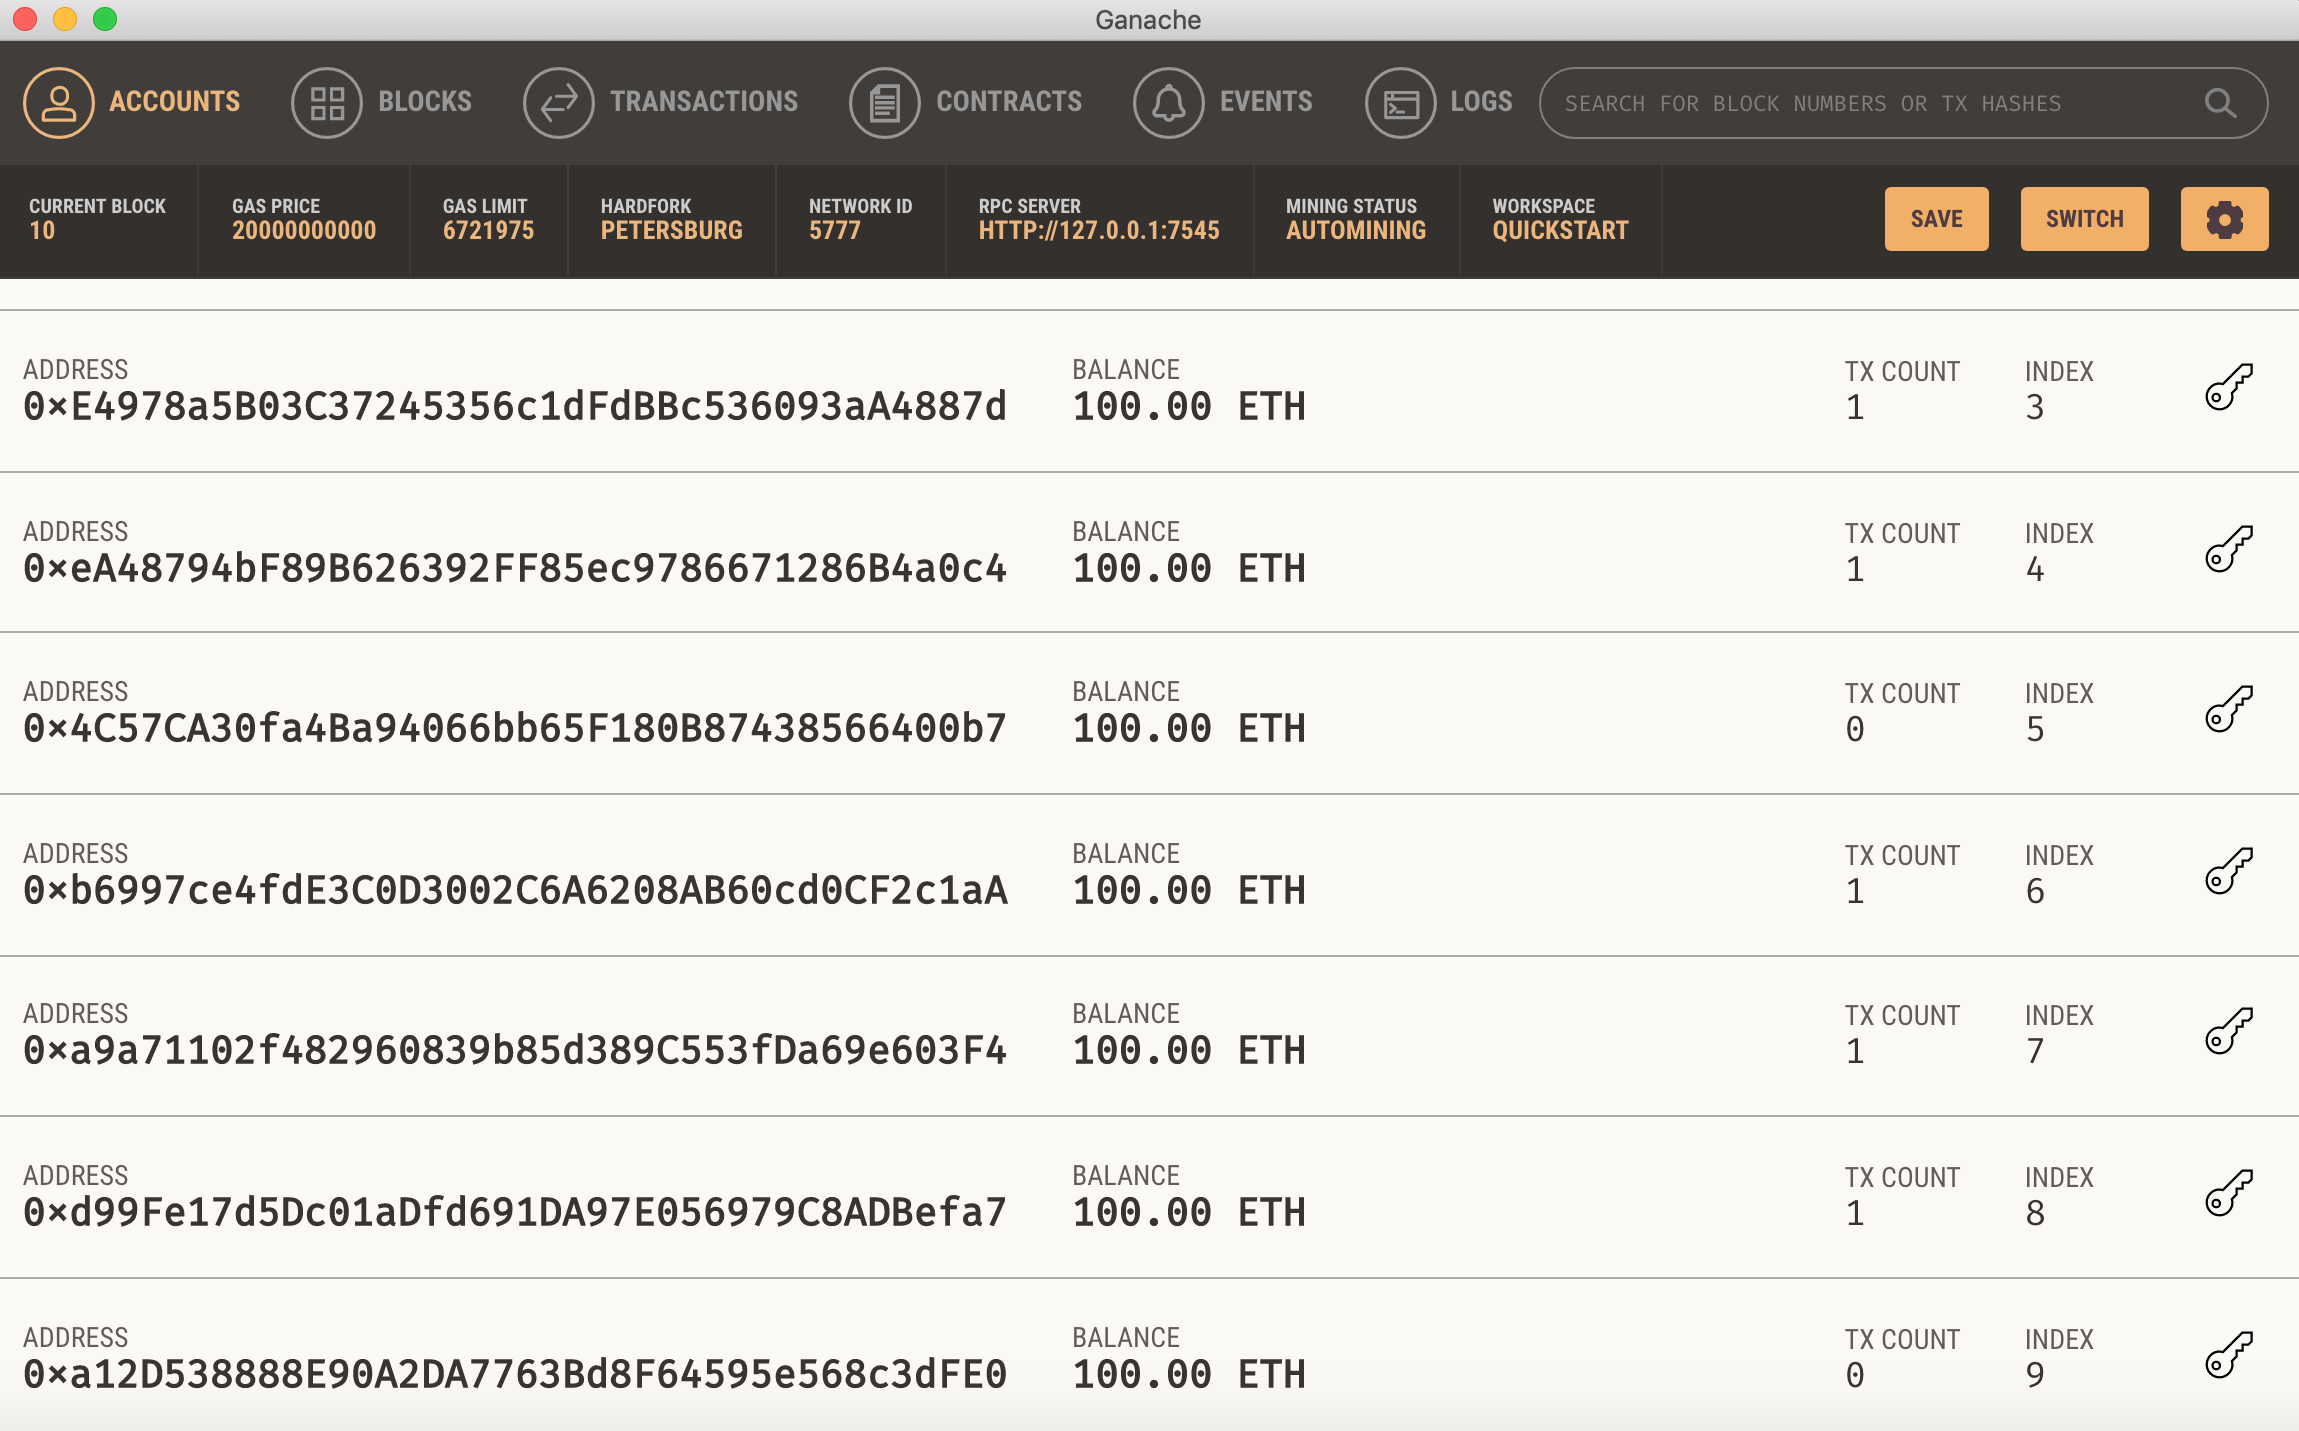
\includegraphics[width=\linewidth]{img/ganache-blockchain.png}
		\caption{Een Lokale blockchain opgezet via Ganache}
		\label{fig:ganache-blockchain}
	\end{figure}
	
	
	\subsection{Metamask}
	Metamask\footnote{Metamask is verkrijgbaar via https://metamask.io of via https://chrome.google.com/webstore} is een Ethereum wallet-plugin voor Google Chrome, die gebruikers in staat stelt om transacties van Ethereum DApps uit te voeren in de browser, zonder zelf een node in het netwerk te moeten zijn. Door Metamask te installeren hoeft men met andere woorden de volledige blockchain dus niet meer te downloaden. 
	
	Voor deze implementatie is Metamask van cruciaal belang, gezien het verantwoordelijk is voor de verificatie van Ethereum-accounts. Daarnaast is het ook een zeer handige tool wanneer we onze implementatie in de browser willen testen, het staat ons toe zeer snel tussen verschillende accounts te schakelen.
	
	Eenmaal de plugin geïnstalleerd is, dient men een paswoord te creëren, daarnaast ontvangt men ook een fallback-sleutel.
	
	\begin{figure}
		
\includegraphics[width=\linewidth]{img/metamask-truffle-ganache.png}
		\caption{Truffle, Metamask en Ganache logo's}
		\label{fig:metamask-truffle-ganache}
	\end{figure}
	\newpage
\section{Implementatie smart contracts}
	Eenmaal alle verschillende tools en plugins uit sectie \ref{sec:benodigdheden} geïnstalleerd zijn, kan men aan het ontwikkelen van smart contracts beginnen. In de volgende subsecties bespreken we de implementatie van een blockchain-gebaseerd stemsysteem op basis van smart contracts. Het volledige project kan worden gevonden op Github\footnote{Zie: https://github.com/Ocean97Li/bachelorproef/tree/master/poc/EthereumVote/backend}. We beginnen met een eenvoudige implementatie die niet \textit{self-tallying} is. In een latere sectie bespreken we wat er nodig is om een veiliger systeem te bekomen.
	\subsection{Opzet Truffle}
	Voor we beginnen met het ontwikkelen van onze smart contracts, moeten we eerst een ontwikkelomgeving opzetten. Voor een vlotte start maken we gebruik van één van de template-projecten beschikbaar via Truffle. 
	
	Na het navigeren naar een gewenste directory gebruikt men het console-commando: 
	 \lstset{language=bash}
	\begin{lstlisting}[numbers=none]
	> truffle unbox pet-shop
	\end{lstlisting}
	
	Dit creëert een nieuw project in de huidige directory. We openen dit in een code-editor (bijvoorbeeld VS-code). Figuur \ref{fig:truffle-template} toont de structuur van de gegenereerde Truffle-template. Het project bevat momenteel zowel een back-end gedeelte (smart contract) als een front-end (javascript project). 
	
	In deze handleiding zullen we - met het principe van herbruikbaarheid in gedachten - de code opsplitsen in afzonderlijke front- en back-end projecten. De folder en inhoud onder \textit{\slash src}, alsook de afbeeldingen \textit{box-img-lg.png} en \textit{box-img-sm.png} mogen dus uit dit project verwijderd worden.
	
	Het project kan nu als start-template worden gebruikt voor onze implementatie.
	
	\begin{figure}
		\centering
		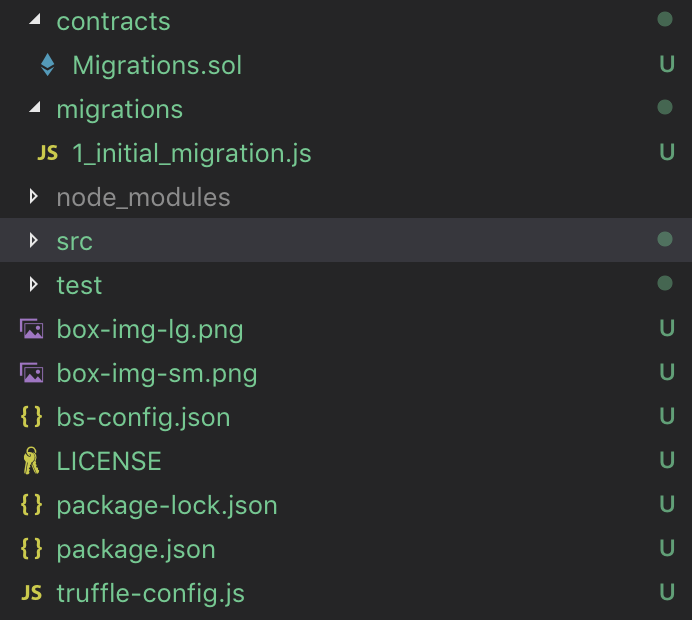
\includegraphics[width=\linewidth/2]{img/truffle-template.png}
		\caption{De structuur van een Ethereum Truffle project}
		\label{fig:truffle-template}
	\end{figure}
	
	\subsection{Basisimplementatie}
	We beginnen met het aanmaken van een nieuw smart contract bestand binnen het template-project. Dit doen we op de locatie \textit{contracts\slash Election.sol}. We overwegen de vereisten voor onze implementatie. Om een simpel stemsysteem te implementeren in een smart contract hebben we nodig:
	\begin{itemize}
		\item een lijst van de `opties' waarop gestemd kan worden
		\item een lijst van de accounts die een stem uitgebracht hebben
		\item per optie het aantal stemmen
	\end{itemize}
	Uiteraard zijn er verschillende manieren waarop we dit kunnen aanpakken. In de context van smart contracts is het echter cruciaal dat we zo weinig mogelijk code schrijven. We baseren ons daarom op de implementatie die wordt gegeven door \textcite{McCubin2019}\footnote{Zie ook https://github.com/dappuniversity/election}.
	
	We beginnen met het declareren van de Solidity-versie:

	\lstset{language=JavaScriptSolidity} 
	\begin{lstlisting}[numbers=none]
	pragma solidity ^0.5.8;
	\end{lstlisting}
	\lstset{language=JavaScriptSolidity} 

	Vervolgens starten we met het definiëren van ons smart contract \textit{Election} :
	\begin{lstlisting}[numbers=none]	
	contract Election {
		constructor () public {
		}
	}
	\end{lstlisting}
	
	Omdat we een lijst van de `opties' willen hebben en ook willen bijhouden per optie hoeveel stemmen er zijn, maken we gebruik van een custom-type dat we \textit{Candidate} noemen. 

	Onze verkiezing hoeft niet per se om het verkiezen van een persoon te gaan, het is echter wel handig om over de opties te denken in termen van`kandidaten'. 
	Iedere optie is een kandidaat die een id, een `naam' (de optie tekst) en een aantal voorkeursstemmen heeft. 
	
	In Solidity definiëren we zo'n custom-type in de vorm van een \textit{struct}:
	
	\begin{lstlisting}[numbers=none]	
	struct Candidate {
		uint id;
		string name;
		uint votes;
	}
	\end{lstlisting}
	
	We breiden \textit{Election} nu ook uit met de volgende attributen:
	
	\begin{lstlisting}[numbers=none]
	//Fetch the candidates	
	mapping(uint => Candidate) public candidates;
	// Store accounts that have voted
	mapping(address => bool) private voters;
	// Read candidate
	uint public candidatesCounter;
	\end{lstlisting}
	
	Het \textit{mapping} keyword in Solidity duidt een hashTable aan, in Solidity is dit de aangeraden verzameling-structuur\footnote{Zie https://ethereum.stackexchange.com/questions/2592/store-data-in-mapping-vs-array\#answer-2597}.  Mappings staan ons toe om key-value searching te doen. In het geval van  \textit{candiates} mappen we de `kandidaten' op basis van hun id's, deze zijn numeriek en incrementeel. We houden het aantal kandidaten bij in \textit{candidatesCounter}, zodat we niet onnodig in de mapping moeten zoeken, maar exact weten wat de range van id's is.
	
	Bij het attribuut \textit{voters} mappen we de adressen van alle kiezers op een booleaanse waarde. Wensen we te weten of een kiezer reeds een stem heeft uitgebracht, dan kunnen we dit via het \textit{voters} attribuut eenvoudig verifiëren. 
	
	We voegen een methode toe aan \textit{Election} die ons in staat stelt om \textit{candiates} te initialiseren:
	
	\begin{lstlisting}[numbers=none]
	function addCadidate(string memory _name) private {
		candidatesCounter++;
		candidates[candidatesCounter] = Candidate(candidatesCounter,_name,0);
	}
	\end{lstlisting}
	Merk op dat de parameter in de bovenstaande functie gemarkeerd is met het Solidity \textit{memory} keyword. Dit duidt aan dat deze parameter niet in de blockchain dient opgeslagen te worden. De tegenhanger van dit keyword is \textit{storage}.
	
	Voorlopig zullen we onze opties `hardcoden' in de constructor-functie, we kiezen voor een implementatie met eenvoudige binaire ja/neen-vragen:
	
	\begin{lstlisting}[numbers=none]
	constructor () public {
		addCadidate("Yes");
		addCadidate("No");
	}
	\end{lstlisting}
	
	Nu we opties hebben toegevoegd waarop gestemd kan worden, rest ons enkel nog het implementeren van een stemfunctie. 
	
	Gebruikers mogen niet meermaals een stem uitbrengen, daarom controleren we iedere gebruiker die probeert te stemmen. 
	
	\begin{lstlisting}[numbers=none]
	function hasVoted() public view returns (bool ok) {
		return voters[msg.sender];
	}
	\end{lstlisting}
	
	Merk ook op dat hier gebruik wordt gemaakt van het Solidity \textit{view} keyword, dit duidt aan dat de betreffende functie geen aanpassingen zal maken aan het contract. 
	
	\begin{lstlisting}[numbers=none]
	function vote(uint _candidateId) public {
		if(!hasVoted()) {
			// Record voter has voted
			voters[msg.sender] = true;
			// Update candidate vote count
			candidates[_candidateId].votes++;
		}
	}
	\end{lstlisting}
	
	We vinden de kandidaat waarvoor de gebruiker stemde op basis van de parameter\textit{\_candidateId}. Door deze waarde in te vullen in de mapping \textit{candidates}, krijgen we toegang tot de correcte Candidate struct. We verhogen het \textit{votes} attribuut van deze struct met 1. Op dit punt is de stem uitgebracht, we hebben nu een eenvoudig stemsysteem bekomen!
	
	De volledige code voor het smart contract \textit{Election.sol} is momenteel:
	
	\lstset{language=JavaScriptSolidity} 
	\begin{lstlisting}[frame=single,  label={lst:election}] 
	pragma solidity ^0.5.8;
	
	contract Election {
		// Store candidate
		struct Candidate {
			uint id;
			string name;
			uint votes;
		}
		//Fetch the candidates
		mapping(uint => Candidate) public candidates;
		// Store accounts that have voted
		mapping(address => bool) private voters;
		// Read candidate
		uint public candidatesCounter;
		
		// Constructor
		constructor () public {
			addCadidate("Yes");
			addCadidate("No");
		}
	
		function addCadidate(string memory _name) private {
			candidatesCounter++;
			candidates[candidatesCounter] = 
			Candidate(candidatesCounter,_name,0);
		}
		
		function hasVoted() public view returns (bool ok) {
			return voters[msg.sender];
		}
		
		function vote(uint _candidateId) public {
			if(!hasVoted()) {
				// Record voter has voted
				voters[msg.sender] = true;
				// Update candidate vote count
				candidates[_candidateId].votes++;
			}
		} // End function
	} // End contract
	\end{lstlisting}
	
	
	\subsection{Migration toevoegen}
	Nu we een functioneel smart contract hebben, wensen we dit op onze lokale blockchain te deployen. Hiertoe dienen we eerst een nieuw migratiebestand aan het project toe te voegen op de locatie \textit{migrations\slash 2\_deploy\_contracts.js}.  
	
	Het nieuwe bestand krijgt de volgende inhoud:
	
	\begin{lstlisting}[frame=single]
	// Find smart contract
	var Election = artifacts.require("./Election.sol");
	
	module.exports = function(deployer) {
	// List all the smart contracts to be deployed
		deployer.deploy(Election);
	};
	\end{lstlisting}
	
	De bovenstaande code zal ervoor zorgen dat Truffle het `Election' smart contract op de blockchain kan plaatsen wanneer we het project deployen.
	
	\subsection{Truffle-project linken aan Ganache}
	
	Om een beter overzicht te krijgen van de `state' van de lokale blockchain, kunnen we ons Truffle-project in Ganache toevoegen. Dit doen we door binnen Ganache naar de menu-optie `Contracts' te navigeren, vervolgens voor de optie `link truffle projects'  te kiezen, naar het project te navigeren en daar het bestand \textit{truffle.js} aan te duiden. Tenslotte  kiezen we voor `save and restart'. Als we nu naar de menu-optie `Contracts' gaan, krijgen we een overzicht van de contracten en hun status (\ref{fig:contracts-ganache1}).
	
	\begin{figure}
		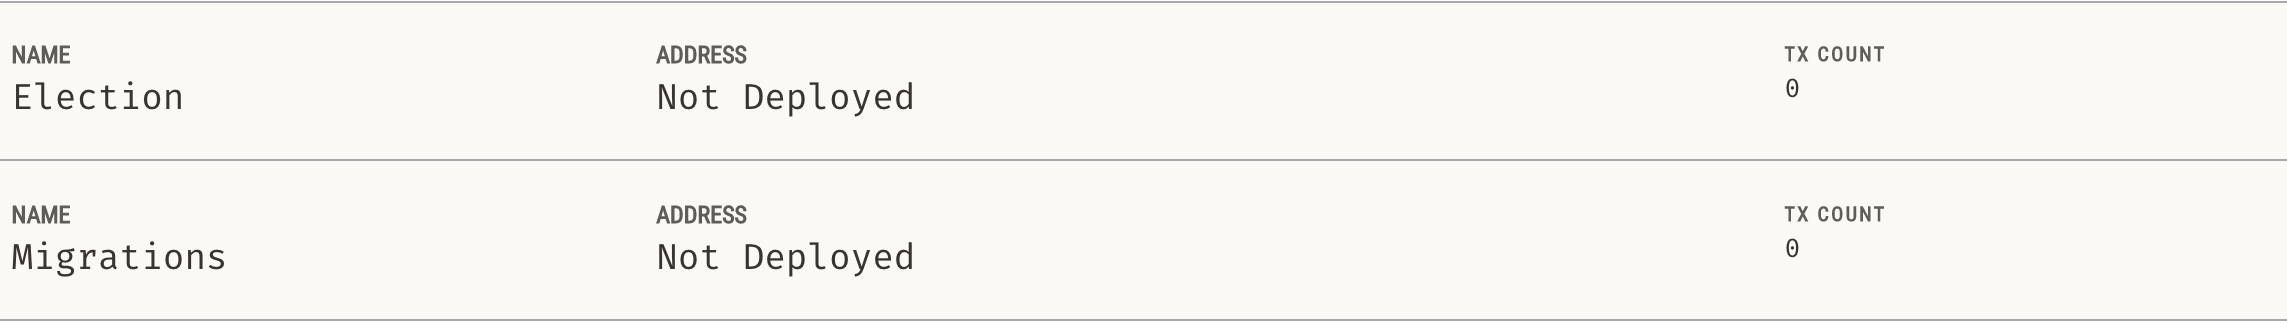
\includegraphics[width=\linewidth]{img/contracts-ganache1.png}
		\caption{De status van smart contracts weergegeven in Ganache}
		\label{fig:contracts-ganache1}
	\end{figure}
	
	
	\subsection{Deployen van smart contracts}
	
	Eenmaal we een migratiebestand voor onze smart contracts hebben, kunnen we deze deployen. Eenmaal de Ganache-blockchain opgestart is en het truffle-project eraan gelinkt, navigeren we naar het project in de console om vervolgens het volgende commando te gebruiken:
	
	\begin{lstlisting}[numbers=none]
	> truffle migrate
	\end{lstlisting}
	
	Merk op dat, indien we nu opnieuw wensen te deployen (in dit geval niet erg omdat we op een lokale blockchain werken), we het volgende commando dienen te gebruiken:
	
	\begin{lstlisting}[numbers=none]
	> truffle migrate --reset
	\end{lstlisting}
	
	Wanneer er geen compilatiefouten aanwezig zijn in de code van de smart contracts, kan er met succes gedeployed worden. In dat geval krijgt men voor elk van de smart contracts een \textit{transaction receipt}:
	\lstset{language=bash}
	\begin{lstlisting}[numbers=none]
	 Deploying `Election'
	--------------------
	> transaction hash:    0xaf22d8d9c9c9a1230e1764d7a3bd9249a3...eb8fa
	> Blocks: 0            Seconds: 0
	> contract address:    0xBF1917F9c9cFee73A4E653de5ad62a6515b78Ed4
	> block number:        3
	> block timestamp:     1560958652
	> account:             0xE03c3692FED9D4f2cBc7c5a30b05Ae9ce7b3b839
	> balance:             99.98553468
	> gas used:            419914
	> gas price:           20 gwei
	> value sent:          0 ETH
	> total cost:          0.00839828 ETH
	
	
	> Saving migration to chain.
	> Saving artifacts
	-------------------------------------
	> Total cost:          0.00839828 ETH
	\end{lstlisting}
	
	Als we de contracts nu in Ganache bekijken, zien we dat de status ook daar veranderd is naar `deployed'. (Zie Figuur \ref{fig:contracts-ganache2})
	
	\begin{figure}
		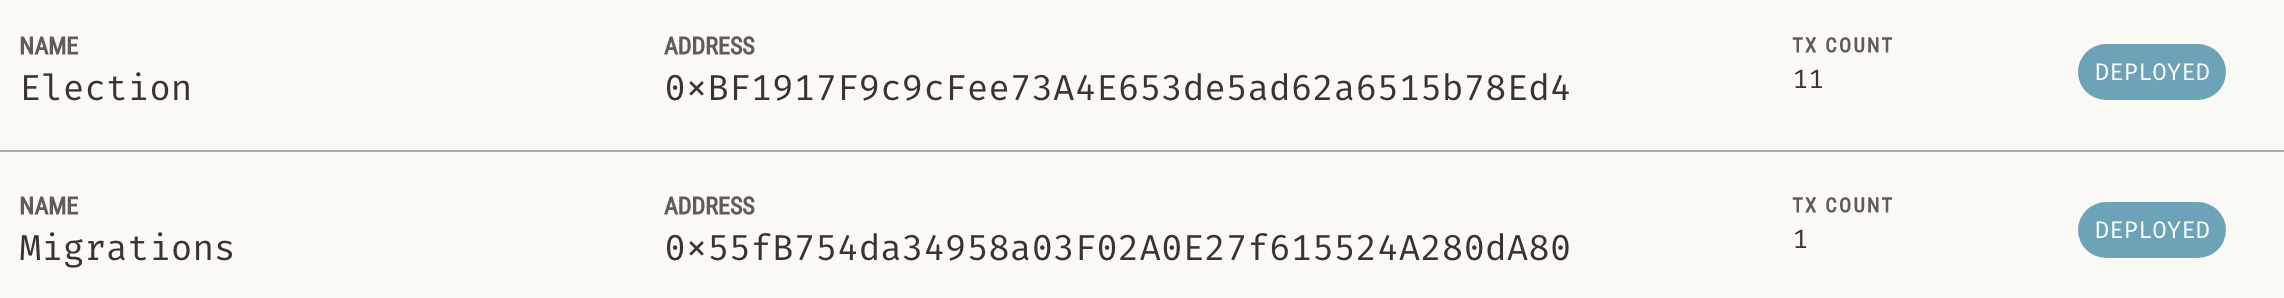
\includegraphics[width=\linewidth]{img/contracts-ganache2.png}
		\caption{Smart contracts `deployed' weergegeven in Ganache}
		\label{fig:contracts-ganache2}
	\end{figure}
	
	\subsection{Belang van testen}
	Bij het ontwikkelen van DApps speelt testen een cruciale rol. Eenmaal gedeployed naar een officieel netwerk, kunnen functies die bugs bevatten en onverwacht gedrag vertonen erg kostelijk zijn voor gebruikers. Het is daarom best practice om enkel smart contracts te deployen die functioneel-volledig en getest zijn.  Doordat alles wat in de blockchain wordt bewaard \textit{immutable} is, betekent het herdeployen van een smart contract eigenlijk dat het huidige contract wordt vervangen door een nieuwe kopie. Zowel de state als het adres van het oude contract gaan verloren. Dit is brekend voor iedere front-end applicatie die aan de DApp verbonden is. 
	
	Door smart contracts grondig te testen kunnen we dergelijke situaties vermijden.
	
	Er zijn verschillende methodes die men kan toepassen om een smart contract te testen, de standaard is om ze te schrijven in Solidity. In dit voorbeeld zullen we echter gebruik maken van Javascript. Via Truffle kunnen we met behulp van Javascript de interacties van gebruikers met onze smart contracts gemakkelijk simuleren. Truffle bevat immers standaard Mocha\footnote{Apart verkrijgbaar via https://mochajs.org} (testframework) en Chai Assertion Library\footnote{Apart verkrijgbaar via https://www.chaijs.com}. Deze twee tools stellen ons in staat om smart contracts te importeren binnenin Javascript-testen. 
	
	\subsection{Smoke test}
	We voegen een nieuw bestand toe op de locatie \textit{test\slash election.js}. We schrijven een smoke test, een test die nagaat of het smart contract op correcte wijze geïnitialiseerd wordt.

	 \lstset{language=JavaScriptSolidity} 
	 \begin{lstlisting}
	 var Election = artifacts.require("./Election.sol");
	 	
	 contract("Election", function(accounts){
		var electionInstance;
		 
		it("Initializes two candidates", function() {
		 	return Election.deployed().then(function(instance){
		 		return instance.candidatesCounter();
		 	}).then(function(count){
		 		assert.equal(count,2);
		 	});
	 	});
	 	
		it("Initializes yes and no", function() {
	 		return Election.deployed().then(function(instance){
	 			electionInstance = instance;
	 			return electionInstance.candidates(1);
	 		}).then(function(candidate){
				assert.equal(
			 	candidate[0],1,"has the correct id: 1"
			 	);
				assert.equal(
				 	candidate[1],"Yes","has the correct value: `Yes'"
				);
				assert.equal(
				 	candidate[2],0,"has the correct amount of votes: 0"
				);
				return electionInstance.candidates(2);
	 		}).then(function(candidate){
				assert.equal(
					candidate[0],2,"has the correct id: 2"
				);
				assert.equal(
					candidate[1],"No","has the correct value: `No'"
				);
				assert.equal(
					candidate[2],0,"has the correct amount of votes: 0"
				);				
	 		}); // End function
	 	}); // End it()
	}); // End contract
	\end{lstlisting}
	
	Concreet testen we hier dat na instantiatie:
	\begin{itemize}
		\item Het attribuut \textit{candidatesCounter} = 2 is.
		\item Het attribuut \textit{candidates[0]} een `kandidaat' is met id = 1, naam = ``Yes'' en aantal stemmen = 0.
		\item Het attribuut \textit{candidates[1]}  een `kandidaat' is met id = 2, naam = ``No'' en aantal stemmen = 0.
	\end{itemize}
	\subsection{Testen uitvoeren}
	Om geschreven testen uit te voeren, navigeren we naar de project-directory en gebruiken we het console-commando:
	
	\begin{lstlisting}[numbers=none]
	> truffle test
	\end{lstlisting}
	
	Truffle voert hierop alle testen binnen de directory \textit{test\slash} uit:
	
	\begin{lstlisting}[numbers=none]
	> Artifacts written to /var/folders/xq/mnnky8qn6c58pt33xhpz2bhw0000gn/T/test-119519-4744-y0zb1c.1il0l
	> Compiled successfully using:
	- solc: 0.5.8+commit.23d335f2.Emscripten.clang
	
	
	
	Contract: Election
	v Initializes two candidates
	v Initializes yes and no (93ms)
	
	
	2 passing (173ms)
	\end{lstlisting}
	
	De smoke test slaagt.
	
	\subsection{Testen in de Truffle console}
	Uiteraard dienen we  ook testen te schrijven voor de stemfunctionaliteit. Gezien dit onderdeel van de code echter nog aan veranderingen onderworpen zal worden, is het misschien voordeliger om de huidige werking op een andere manier te verifiëren. In plaats van een test te schrijven, kunnen we via de \textit{Truffle console} de toestand van de lokale blockchain bekijken.
	
	In de console navigeren we naar het project, vervolgens gebruiken we het console-commando:
	
	\begin{lstlisting}[numbers=none]
	> truffle console
	\end{lstlisting}
	
	Dit opent de Truffle-console. 
	Hier geven we het volgende commando in:

	\begin{lstlisting}[numbers=none]
	truffle(development)> Election.deployed()
		.then(function(i){app = i})
	\end{lstlisting}
	
	Indien het Election contract gedeployed is, wordt er een asynchrone callback-functie uitgevoerd.  De functie in kwestie krijgt  een instantie van Election (i) mee als parameter en maakt deze toegankelijk door ze in een variabele op te slaan. Eenmaal de asynchrone code uitgevoerd is, hebben we via \textit{app} toegang tot de attributen en functies van het smart contract Election.
	
	Gezien we de stemfunctionaliteit willen testen, zullen we de stemfunctie \textit{vote()} oproepen.
	
	Hiervoor hebben we echter het publieke adres van een van de Ganache-accounts nodig. Deze kan men vinden in Ganache zelf, of men kan ze bekomen via het Truffle console-commando:
	\begin{lstlisting}[numbers=none,language=bash]
	truffle(development)>web3.eth.getAccounts()
	[ `0xE03c3692FED9D4f2cBc7c5a30b05Ae9ce7b3b839',
	`0xe60c19f8a1baC541483e303Dc3d9B4e28d580980',
	`0x47B7B70802E9eC6a5Df8570962574894f0Ac4c15',
	`0xE4978a5B03C37245356c1dFdBBc536093aA4887d',
	`0xeA48794bF89B626392FF85ec9786671286B4a0c4',
	`0x4C57CA30fa4Ba94066bb65F180B87438566400b7',
	`0xb6997ce4fdE3C0D3002C6A6208AB60cd0CF2c1aA',
	`0xa9a71102f482960839b85d389C553fDa69e603F4',
	`0xd99Fe17d5Dc01aDfd691DA97E056979C8ADBefa7',
	`0xa12D538888E90A2DA7763Bd8F64595e568c3dFE0' ]
	\end{lstlisting}
	
	We kopiëren een adres naar keuze en vullen dit in als de \textit{from} property van het object dat de tweede parameter vormt. Op deze manier versturen we een transactie vanuit de console, in naam van het geselecteerde adres. De eerste parameter is het id van de `kandidaat' waarvoor we stemmen.
	\begin{lstlisting}[numbers=none,language=bash]
	truffle(development)> app.vote(1, 
		{ from: `0xE03c3692FED9D4f2cBc7c5a30b05Ae9ce7b3b839'}
	)
	\end{lstlisting}
	
	Ook hier krijgen we een \textit{transaction receipt}.
	Om te controleren of er een stem is bijgekomen voor de gekozen optie, geven we de volgende Truffle console-commando's in:
	\begin{lstlisting}[numbers=none]
	truffle(development)> app.candidates(1)
	truffle(development)> app.candidates(2)
	\end{lstlisting}
	Dit resulteert in:
	\begin{lstlisting}[numbers=none,language=bash]
	Result {												Result {
	...															...
	id: <BN: 1>,										id: <BN: 2>,
	name: `Yes',									  name: `No',
	votes: <BN: 1> }							  votes: <BN: 0> }
	\end{lstlisting}
	
	Voor de eerste optie (`Yes') zien we dat er onder het attribuut \textit{votes} de waarde <BN: 1> staat. Het aantal stemmen hier is met andere woorden 1.
	Voor de tweede optie (`No') is dat niet het geval, \textit{votes} heeft de  waarde <BN: 0>. Het aantal stemmen hier dus onveranderd, 0.
	
	Dit toont aan dat onze stemfunctie wel degelijk werkt! 
	
	Figuur \ref{fig:contracts-ganache3}: Ook in Ganache zien we dat er een nieuwe transactie heeft plaatsgevonden. Merk wel op dat de huidige implementatie totaal geen garantie biedt op het vlak van anonimiteit (aan de hand van de input van iedere transactie kunnen we het stemgedrag van iedere kiezer afleiden). Het enige wat de anonimiteit van een kiezer enigszins beschermt, is de abstracte aard van de accounts: de kiezer is alleen bekend via zijn Ethereum-adres. 
	\begin{figure}
		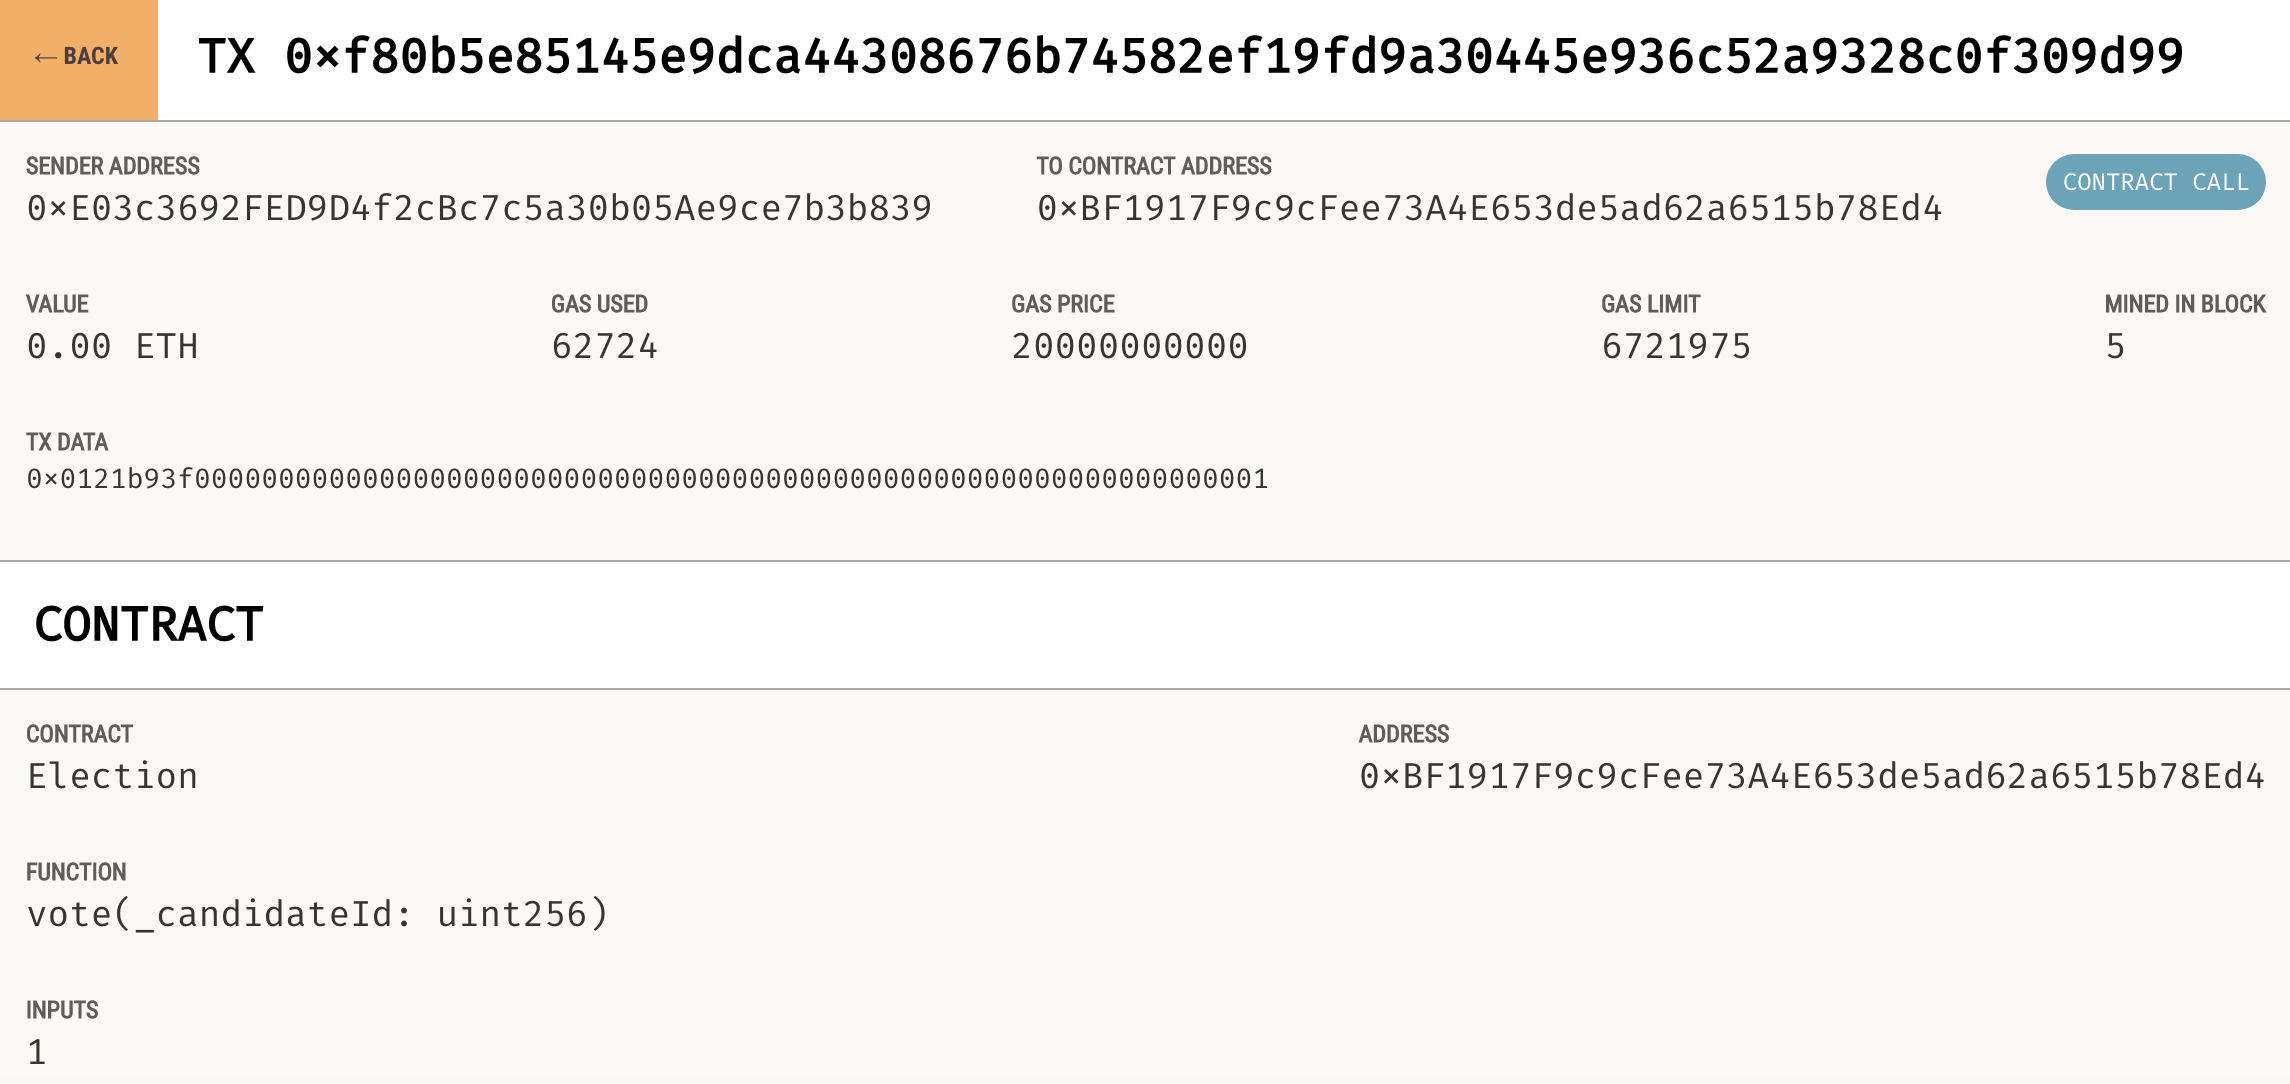
\includegraphics[width=\linewidth]{img/contracts-ganache3.png}
		\caption{Vote functie aangeroepen weergegeven in Ganache}
		\label{fig:contracts-ganache3}
	\end{figure}
	\newpage
	\section{Front-end applicatie}
	Eenmaal we een werkende back-end hebben, dienen we er natuurlijk ook nog een front-end applicatie voor te ontwikkelen. In deze handleiding zullen we gebruik maken van Angular (figuur \ref{fig:angular}), een open source javascript-framework dat ontwikkelaars in staat stelt performante \textit{single page applications} te schrijven. We verkiezen Angular omdat de structurering van de code bijzonder vast is in dit framework, waardoor de functionaliteiten mooi opgesplitst zijn en de ontwikkelervaring bijzonder aangenaam is.  Het staat de lezer natuurlijk vrij om een javascript-framework naar keuze te gebruiken. Het gaat hier immers niet zo zeer om de ontwikkeling van de front-end applicatie als om het leggen van de verbinding tussen het web en de Ethereum-blockchain...
	\begin{figure}[h!]
		\centering
		
\includegraphics[width=\linewidth/3]{img/angular.png}
		\caption{Het Angular logo ~\autocite{Angular2019}}
		\label{fig:angular}
	\end{figure}
	\subsection{Opzet}
	Zoals gezegd beginnen we met een Angular project op te zetten, lezers die gebruik maken van een ander Javascript-framework kunnen de volgende stappen overslaan, zij hoeven enkel de vernoemde node\_modules te installeren en de code gegeven in de \textit{ElectionConnectorService} te herschrijven. 
	
	We beginnen met het installeren van de Angular cli, deze zal ons toestaan een Angular project te maken.
	
	We maken gebruik van het console-commando:
	\begin{lstlisting}[numbers=none,language=bash]
	>npm install -g @angular/cli
	\end{lstlisting}
	Dit installeert de Angular cli op een globaal niveau, vanaf nu kunnen we er overal gebruik van maken.
	
	We navigeren naar de directory waar we het front-end project willen aanmaken, vervolgens gebruiken we het console-commando:
	\begin{lstlisting}[numbers=none,language=bash]
	>ng new EthereumVote
	\end{lstlisting}
	De Angular cli zal nu een nieuw project voor ons creëren in de huidige directory. 
	
	Nu installeren we de nodige node\_packages:
	\begin{itemize}
		\item \textbf{web3.js}: een verzameling javascript libraries  die het mogelijk maken om te communiceren met Ethereum-instanties, hetzij via  een HTTP-, webSocket- of IPC-verbinding. Web3 bevat in feite alles wat nodig is om de front-end van een DApp te ontwikkelen.
		\item \textbf{truffle-contract}: maakt een lokale interface van het smart contract aan, waarmee we kunnen interageren in de front-end. Het aanmaken van de instantie gebeurt op basis van het gecompileerde smart contract in json-format.
	\end{itemize}

	\subsection{Mogelijke problemen met Web3}
	
	Na de installatie van web3.js is het mogelijk dat men problemen ervaart met verschillende node\_modules die niet kunnen gevonden worden. Voor lezers die problemen ervaren met onder andere de \textit{crypto}, \textit{streams} of \textit{http } modules is het aangeraden om een van de volgende oplossingen te proberen:
	\begin{itemize}
		\item Patch file voor de node\_modules
		\item Downgraden naar \textit{web3.js versie 0.20.5}. 
	\end{itemize}
	
	In deze handleiding raden we aan om de oplossing met het \textit{patchfile.js}\footnote{Broncode: https://gist.github.com/niespodd/1fa82da6f8c901d1c33d2fcbb762947d} als eerste te proberen:
	\begin{lstlisting}[numbers=none,language=bash]
	const fs = require("fs");
	const f = "node_modules/@angular-devkit/build-angular
	/src/angular-cli-files/models/webpack-configs/browser.js";
	fs.readFile(f, "utf8", function (err,data) {
		if (err) return console.log(err);
		var result = data.replace(/node: false/g, "node: {crypto: true, stream: true}");
		fs.writeFile(f, result, "utf8", function (err) {
			if (err) return console.log(err);
		});
	});
	\end{lstlisting}
	Deze code dient na iedere wijzing van de node\_modules te worden uitgevoerd, onder \textit{``scripts''} in de \textit{package.json} voegen we daarom toe:
	\begin{lstlisting}[numbers=none,language=bash]
	"scripts": {
	...
	"postinstall": "node patch.js"
	},
	\end{lstlisting}
	
	Enkel en alleen als de eerste optie niet werkt, raden we aan om web3 te downgraden. Het is de lezer aangeraden om over te schakelen naar yarn package manager ten voordele van npm. Yarn kan beter overweg met het toevoegen, verwijderen en onderhouden van dependencies. Ook voor gebruikers die geen verdere problemen meer ondervinden met web3, kan het daarom waardevol zijn om yarn te installeren. Yarn- en npm-commando's zijn helemaal gelijk, op de begin-keywords na. In de rest van deze handleiding wordt er gebruik gemaakt van yarn-commando's.
	
	Eenmaal yarn\footnote{Verkrijgbaar via https://yarnpkg.com/lang/en/docs/install} geïnstalleerd is, kunnen console-commando's gebruikt worden om web3 te herstellen:
	\begin{lstlisting}[numbers=none,language=bash]
	>yarn
	>yarn remove web3
	>yarn add web3@0.20.5
	\end{lstlisting}

	\subsection{Mogelijke problemen met Truffle-Contract}
	Lezers die problemen ondervinden bij de  installatie van de \textit{truffle-contract} module, installeren het best versie v4.0.20. Bij aanhoudende problemen kan men de nodige \textit{yarn.lock }en \textit{package.json} op de Github-pagina\footnote{Zie https://github.com/Ocean97Li/bachelorproef/blob/master/poc/EthereumVote/frontend/yarn.lock} van het project vinden. De meeste problemen met \textit{node\_packages} kunnen opgelost worden door deze twee configuratiebestanden in het lokale project te vervangen door de bestanden die op Github staan. Vervolgens dient men nog eens gebruik te maken van het yarn-commando.
	
	\subsection{Algmenene structuur EthereumConnector}
	Eenmaal de nodige zaken geïnstalleerd zijn, kunnen we beginnen met de implementatie van een stemsysteem. Zoals gezegd zal de focus hier voornamelijk liggen op het implementeren van de functionaliteiten in verband met  de Ethereum-netwerkverbinding. Voor de herbruikbaarheid en performantie worden alle functionaliteiten in een service gebundeld,  zoals gebruikelijk binnen Angular. De code voor de rest van de applicatie (voornamelijk de visuele componenten en verschillende schermen) wordt enkel kort besproken.  Eenmaal de service geïmplementeerd is, staat het de lezer natuurlijk vrij om er direct zelf mee aan de slag te gaan en er een applicatie rond te ontwikkelen.
	
	 We beginnen met het aanmaken van de \textit{EthereumConnectionService.} 
	
	We maken een nieuw bestand aan op de locatie \textit{services/ethereum-connector.service.ts} via de console-commando's:
	\begin{lstlisting}[numbers=none,language=bash]
	>mkdir services
	>cd services
	>ng generate service EthereumConnector
	\end{lstlisting}
	
	Dit geeft ons een service-template waarmee we kunnen starten met ontwikkelen.
	
	We overlopen eerste de grote functionaliteiten die we wensen te implementeren:
	\begin{itemize}
		\item \textbf{vote()}: Een stemfunctie die toestaat de gelijknamige functie in het smart contract \textit{Election} aan te spreken. Het id van de gewenste kandidaat moet als parameter worden mee gegeven.
		\item \textbf{register()}: Een stemfunctie die toestaat  de gelijknamige functie in het smart contract \textit{Election} aan te spreken. Ook hier moet het id van de gewenste kandidaat worden mee gegeven als parameter.
		\item \textbf{getVotes()}: Eenmaal een stem is uitgebracht, willen we de resultaten van de verkiezing visualiseren. Hiervoor moeten we het attribuut \textit{candidates} van \textit{Election} retourneren.
		\item \textbf{checkVotedYet()}: Functie die het \textit{votedVoters} attribuut van \textit{Election} aanspreekt en weergeeft of een kiezer al dan niet een stem heeft uitgebracht.
		\item \textbf{getCandidates()}: Haalt de kandidaten en hun \textit{id}'s op. De namen worden gebruikt om weer te geven, de id's vormen de achterliggende opties waarop men kan stemmen.
		\item \textbf{getAccountInfo()}: Controleert via web3 of er een Ethereum-account is ingelogd in de browser en of het account genoeg ether heeft om te registreren en en te stemmen.
		\item \textbf{truffleContract()}: Initieert een interface van \textit{Election} op basis van het gecompileerde smart contract. Via deze interface kunnen we  interageren met smart contracts.
	\end{itemize}

Daarnaast zijn er ook een heel aantal velden om verschillende zaken bij te houden. 

Tabel \ref{tab:ethservice} geeft een overzicht van de verschillende attributen die we zullen gebruiken om zaken bij te houden in de connectorService. 
Merk op dat er voor veel van de private domeinattributen (die te maken hebben met stemmen) gelijknamige publieke attributen van het type Subject zijn. Externe componenten kunnen de methode \textit{subcribe()} van deze attributen oproepen  om op de hoogte te worden gehouden van specifieke veranderingen aan de private domeinattributen van de connectorService. Via de Subjects kunnen we de veranderingen doorsturen naar de verschillende componenten die hiervan afhankelijk zijn.

	\begin{table}
		\centering
		\begin{tabular}{ |l|c|c|c| } 
			\hline
			\textbf{property naam} & \textbf{toegankelijkheid}&  \textbf{type}  \\
			\hline
			electionInstance 		& private & null \\ 
			web3Provider 			& private & number\\ 
			account 					  & private & string \\ 
			votingKey 					& private & string \\ 
			votes 							 & private & Map<string, number> \\ 
			candidates 					& private & Map<string, number>  \\ 
			refreshVotes\$ 			 & private & Observable<number>  \\ 
			state 							  & private & ElectionState  \\ 
			account\$  					& public & Subject<string> \\ 
			votes\$  					   & public & Subject<Map<string, number> > \\ 
			candidates\$ 			 & public & Subject<Map<string, number> > \\ 
			state\$ 						& public & Subject<ElectionState>  \\ 
			error\$ 						& public & Subject<string> \\ 
			\hline
		\end{tabular}
	\caption{Attributen en hun type binnen de EthereumConnectorService}
	\label{tab:ethservice}
\end{table}
\newpage
\subsection{Bespreking verschillende methodes}
	\subsubsection{truffleContract}
	\lstset{language=JavaScriptSolidity} 
	\begin{lstlisting}[numbers=none]
	import * as TruffleContract from 'truffle-contract';
	...
	const tokenAbi = require('../../../backend/build/contracts/Election.json');
	...
	get truffleContract() {
		if (!this.contract) {
			const contract = TruffleContract(tokenAbi);
			contract.setProvider(this.web3Provider);
			this.contract = contract;
		}
		return this.contract;
	}
	\end{lstlisting}
	De getter-functie \textit{truffleContract()} maakt met behulp van de  truffle-contract bibliotheek een nieuwe interface aan om het smart contract te creëren. De parameter \textit{tokenAbi} geeft het pad naar het gecompileerde \textit{Election.json} smart contract in de back-end. Merk ook op dat deze methode de \textit{lazy-loading} filosofie volgt: zolang het contract niet wordt aangeroepen, wordt het ook niet geïnitialiseerd.
	\subsubsection{getAccountInfo}
	\lstset{language=JavaScriptSolidity} 
	\begin{lstlisting}[numbers=none]
	private getAccountInfo() {
		return new Promise((resolve, reject) => {
			window.web3.eth.getCoinbase((err, account) => {
				if (err === null && account !== null) {
					this.account = account;
					window.web3.eth.getBalance(account, (error, balance) => {
						if (error === null && balance > 0) {
							return resolve();
						} else {
							return reject();
						}
					});
				} else {
					return reject();
				}
			});
		});
	}
	\end{lstlisting}
	 \textit{GetAccountInfo()} is de methode die wordt gebruikt voorafgaand aan iedere transactie om het Ethereum-account op te halen en te controleren. We werken hier (zoals meestal) met een ketting van opeenvolgende en geneste \textit{promises}. We beginnen bij het begin: de initialisatie van een nieuwe promise als retourwaarde. Wanneer men een promise declareert, zijn er twee zaken die in de callback-functie kunnen gebeuren:  ofwel wordt de methode \textit{reject()} aangeroepen en stopt de ketting van promises op dat punt, ofwel wordt \textit{resolve()} aangeroepen en gaat men verder naar de volgende promise.
	\subsubsection{getCandidates}
	\lstset{language=JavaScriptSolidity} 
	\begin{lstlisting}[numbers=none]
	public getCandidates() {
		this.truffleContract.deployed().then((instance) => {
			this.electionInstance = instance;
			return this.electionInstance.candidatesCounter();
		}).then((candidatesCounter) => {
			this.candidatesCounter = candidatesCounter;
			return this.findEachCandidateIds();
		}).then(() => {
			this.candidates$.next(this.candidates);
		}).catch((error) => {
			this.error$.next(error);
			console.log(error);
		});
	}
		
	private findEachCandidateIds() {
		return new Promise((resolve, reject) => {
			const promises = [];
			const number = this.candidatesCounter.toNumber();
			for (let i = 1; i <= number; i++) {
				promises[i] = this.electionInstance.candidates(i)
				.then((candidate) => {
					this.candidates.set(
						candidate[0].toNumber(),
						candidate[1]
					);
				});
			}
			Promise.all(promises).then(() => {
					resolve();
				});
			});
		}
		\end{lstlisting}
		Voor we effectief kunnen stemmen, moeten we weten uit welke opties kan gekozen worden. Tot dat doeleinde dienen de methodes \textit{getCandidates} en \textit{findEachCandidateIds}. Deze zorgen ervoor dat de mogelijke `kandidaten' opgevraagd worden van het smart contract. 
		
		De eerste stap is het ophalen van een nieuwe \textit{electionInstance}. Eenmaal dit voltooid is, bevragen we het smart contract voor de \textit{candidatesCounter}. Wanneer vervolgens ook dit getal binnen is, overlopen we iedere kandidaat in \textit{findEachCandidateIds()} aan de hand van de \textit{candidatesCounter}. We bewaren enkel de eerste twee attributen:  naam en id. Voor iedere kandidaat maken we een asynchrone call naar het smart contract. Het resultaat van iedere call (per kandidaat) slaan we op in een array van promises.
		
		Met \textit{Promise.all(promises)} verzekeren we ons ervan dat de promise die in \textit{findEachCandidateIds()} gemaakt wordt pas de \textit{resove()} uitvoert op het moment dat we een naam en id voor iedere kandidaat hebben.
		
		Tenslotte stellen we alle luisterende componenten via \textit{candidates\$} op de hoogte. 
	\subsubsection{checkVotedYet}
	\lstset{language=JavaScriptSolidity} 
	\begin{lstlisting}[numbers=none]
	public checkVotedYet() {
		return new Promise( (resolve, reject) => {
			return this.truffleContract.deployed().then((instance) => {
				this.electionInstance = instance;
				return this.electionInstance.hasVoted({from:this.account});
			}).then((voted) => {
				if (voted) {
					setTimeout( () => {
						window.alert('It seems you have already voted!');
						this.state = ElectionState.verified;
						this.state$.next(this.state);
					}, 2000);
				}
			}).then(() => {
				resolve();
			}).catch((error) => {
				this.error$.next(error);
				reject();
			});
		});
	}
	\end{lstlisting}
	In onze verkiezing is het uiteraard niet wenselijk dat een persoon meerdere malen kan stemmen. Om dit tegen te gaan, voorzagen we reeds een nodige check bij de vote-functie in de back-end. In de front-end willen we echter onnodig werk en transactiekosten voor de gebruiker vermijden door het aanroepen van de stemfunctionaliteit op bepaalde momenten te verhinderen. 
	
	Via de methode \textit{checkVotedYet()} kunnen we exact dat doen: we vragen het smart contract eenvoudigweg of de gebruiker in kwestie al gestemd heeft.
	\subsubsection{getVotes}
	\lstset{language=JavaScriptSolidity} 
	\begin{lstlisting}[numbers=none]
	private refreshVotes$: Observable<number> = timer(0, 2000);
	...
	public async getVotes() {
		this.truffleContract.deployed().then((instance) => {
			this.electionInstance = instance;
			return this.electionInstance.candidatesCounter();
		}).then((candidatesCounter) => {
			this.candidatesCounter = candidatesCounter;
			return this.findEachCandidateVotes();
		}).then(() => {
			this.votes$.next(this.votes);
		}).catch((error) => {
			this.error$.next(error);
			console.log(error);
		});
	}
	...
	this.refreshVotes$.subscribe(() => {
		this.getVotes().catch();
	});
	\end{lstlisting}
	Zodra een stem is uitgebracht, willen we in onze implementatie het (tussentijdse) resultaat van de verkiezing zien. Gezien er ondertussen mogelijks andere kiezers hun stem hebben uitgebracht, dienen we de resultaten regelmatig te hernieuwen. Tot dat doeleinde wordt de asynchrone functie \textit{getVotes()} gedefinieerd. Voor het regelmatig ophalen van stemmen gebruiken we \textit{refreshVotes\$}, deze property bevat een \textit{observable timer}. De callback-functie zal na het aanroepen van \textit{subscribe(callback)} elke twee seconden worden uitgevoerd. We roepen er \textit{getVotes()} op.
	\subsubsection{register}
	\lstset{language=JavaScriptSolidity} 
	\begin{lstlisting}[numbers=none]
	public register() {
		return new Promise((resolve, reject) => {
			return this.truffleContract.deployed().then((instance) => {
				this.electionInstance = instance;
				return this.getAccountInfo();
			}).then(() => {
				return this.electionInstance.hasRegistered({from: this.account});
			}).then((registered) => {
				if (registered) {
					this.state = ElectionState.loggedin;
					this.state$.next(this.state);
					throw Error('already registered');
				}
			}).then(() => {
				this.votingKey = (Math.floor(Math.random() * 99) + 1).toString();
				return this.electionInstance.register(window.web3.sha3(this.votingKey), {from: this.account})
					.then(() => {
						this.state = ElectionState.loggedin;
						this.state$.next(this.state);
					});
				}).then(() => {
					resolve();
				}).catch((error) => {
					this.error$.next(error);
					reject(error);
				});
		}).catch((error) => {
			if (error === 'already registered') {
				console.log(error);
			}
			this.error$.next(error);
		});
	}
	\end{lstlisting}
		Vooraleer gebruikers een stem mogen uitbrengen, wensen we dat ze zich registreren als kiezer. Bij de registratie genereren kiezers een unieke stemsleutel met een cijfer dat alleen zij kennen. Deze sleutel wordt doorgegeven aan het smart contract en daar opgeslagen. Wanneer gebruikers een stem moeten uitbrengen, wordt hen gevraagd om het geheime cijfer bekend te maken (commit-reveal pattern). In het smart contract zal er vervolgens gecontroleerd worden of de stemsleutel kan gereproduceerd worden met dat cijfer. Is dit het geval, dan weten we met zekerheid dat we met een legitieme kiezer te maken hebben, de stem van de kiezer wordt geregistreerd.
		
		De methode begint met het initialiseren van de \textit{electionInstance}, vervolgens wordt \textit{getAccoutInfo()} aangeroepen. Wanneer \textit{getAccoutInfo()} voltooid is, wordt de \textit{hasRegistered} op de \textit{electionInstance} aangeroepen. Als de gebruiker in kwestie reeds geregistreerd is, wordt er een error geworpen om de promise-ketting te doorbreken. Indien de gebruiker nog niet geregistreerd was, gaat de promise-ketting gewoon verder. Er wordt een stemsleutel voor de gebruiker gegenereerd. Dit gebeurt via het een random getal dat door de \textit{web3Provider} gehashed wordt met een \textit{sha3-hash} (de web3 sha3-hash is dezelfde als de \textit{keccak256-hash} in Solidtiy).
		
		De stemsleutel wordt meegegeven als parameter in \textit{register()}, de functie die wordt opgeroepen op de \textit{electionInstance}.
	\subsubsection{vote}
	\lstset{language=JavaScriptSolidity} 
	\begin{lstlisting}[numbers=none]
	public vote(candidate: string) {
		this.state = ElectionState.voted;
		this.state$.next(this.state);
		this.checkVotedYet().then(() => {
			if (this.state.valueOf() < ElectionState.verified.valueOf()) {
				this.truffleContract.deployed().then((instance) => {
					this.electionInstance = instance;
				}).then(() => {
					return this.getAccountInfo();
				}).then(() => {
					return this.electionInstance.hasRegistered({from: this.account});
				}).then((registered) => {
					if (!registered) {
						throw Error('not registered');
					}
					return this.electionInstance.hasVoted({from: this.account});
				}).then((voted) => {
					if (voted) {
						throw Error('already voted');
					}
					this.state = ElectionState.voted;
					this.state$.next(this.state);
					return this.electionInstance.vote(candidate, this.votingKey, {from: this.account});
				}).then(() => {
					this.state = ElectionState.verified;
					this.state$.next(this.state);
				}).catch((error) => {
					console.log(error);
				});
			}
		});
	}
	\end{lstlisting}
	Wanneer kiezers hun stem uitbrengen zijn er een heleboel zaken die gecontroleerd dienen te worden. 
	
	Als eerste controleren we via \textit{checkVoted()} of het huidige account al dan niet reeds gestemd heeft. Accounts die aan deze stap voldoen krijgen een melding en worden vervolgens direct naar de resultaten-pagina gestuurd.
	
	Via \textit{getAccountInfo()} wordt vervolgens de validiteit van het ingelogde account gecontroleerd (correct ingelogd en geen lege portefeuille). Accounts die niet aan deze controle voldoen worden geweerd. 
	
	Accounts die voor het eerst een stem mogen uitbrengen en over een geldig en ingelogd account beschikken, worden gecontroleerd op registratie. Niet-geregistreerde accounts worden geweerd, geregistreerde accounts worden nu als kiezers gezien.
	
	Een kiezer is iemand die aan alle voorwaarden voldoet. Deze persoon kan een stem uitbrengen via \textit{vote()}. Het geheime getal dat gebruikt werd om de stemsleutel te genereren tijdens het registreren (attribuut \textit{votingKey}), wordt nu samen met het id van de gekozen kandidaat als parameter meegegeven aan de \textit{vote()} functie van \textit{electionInstance}.
	\subsection{Veranderingen in de state}
	De attente lezer merkte  doorheen de code waarschijnlijk verschillende statements op, zoals \textit{this.state = ElectionState.voted} en \textit{this.state\$.next(this.state)}. Dit zijn wijzigingen aan de interne staat van de applicatie. We gebruiken \textit{this.state} om de lokale vooruitgang binnen het verkiezingsproces bij te houden, via \textit{this.state\$.next(this.state)} verwittigen we alle \textit{listeners} (inclusief de connector zelf) van de gemaakte verandering.
	
	De statussen delen het stemproces op in verschillende sequentiële stappen, we definiëren:
	\begin{lstlisting}[numbers=none]
	export enum ElectionState {
		notloggedin,
		loggedin,				
		voted, 						
		verified  					 
	}
	\end{lstlisting}
	De voornaamste reden waarvoor \textit{state} gebruikt wordt, is om de vooruitgang binnen het stemproces visueel weer te geven doorheen de verschillende schermen in de applicatie. Concreet gebruiken we de veranderingen in \textit{state} om de \textit{component routing} te besturen: bij iedere verandering van \textit{state} wordt de \textit{Angular Router} aangeroepen om naar een nieuw scherm te navigeren.
	
	Normaal gezien is het uitvoeren van \textit{routing} iets wat alleen ter hoogte van de componenten gebeurt, maar in dit geval (voor de volledigheid en herbruikbaarheid van de code) lijkt het beter om dit binnen de \textit{EthereumConnectorService} te implementeren. 
	
	Opdat de routing probleemloos zou werken buiten een component (zonder irregulier gedrag), dienen we gebruik te maken van een \textit{wrapping} van de code met \textit{ngZone.run()}.
	
	De code die zorgt voor automatische routing bij verandering van \textit{state} is de volgende:
	\begin{lstlisting}[numbers=none]
	this.state$.subscribe( state => {
		let route: string;
		switch (state) {
			case ElectionState.notloggedin:
			route = "login";
			this.register(); break;
			case ElectionState.loggedin:
			route = "vote"; break;
			case ElectionState.voted:
			route = "verify"; break;
			case ElectionState.verified:
			route = "results"; break;
		}
		this.router.navigateByUrl(`/${route}`);
	});
	\end{lstlisting}
	Voor iedere verandering in \textit{electionState} is er een corresponderende route.
	
	De routes \textit{(`login',`vote',`verify',`results')} definiëren en injecteren we in \textit{app.module.ts}:
	\begin{lstlisting}[numbers=none]
	const routes: Route[] = [
		{path: "vote", component: VotingComponent},
		{path: "results", component: ResultsComponent},
		{path: "login", component: LoginComponent},
		{path: "verify", component: VerifyComponent},
		{path: "**", component: LoginComponent}
	];
	
	@NgModule({
		...
		imports: [
			...
			RouterModule.forRoot(routes),
			...
		]
	})
	\end{lstlisting}
	\subsection{Componenten}
	Tot slot geven we een kort overzicht van de verschillende componenten die gebruikt worden in deze applicatie. Iedere component stemt overeen met één scherm in de DApp en één stap in het verkiezingsproces. 
	
	Merk op dat de onderstaande HTML5-code specifiek is geschreven binnen de context van het Angular Framework. Gebruikers die een zelf een front-end wensen te ontwikkelen via een ander framework of zonder framework, kunnen zich enkel op deze code baseren, maar niet letterlijk overnemen. 
	
	De volledige implementatie is te vinden op Github\footnote{https://github.com/Ocean97Li/bachelorproef/tree/master/poc/EthereumVote/frontend/src/app/components}.
	\newpage
	\subsubsection{Login}
	In \textit{app/components/login/login.html}
	\begin{lstlisting}[frame=single,language=HTML5]
	<div class="card">
		<h1>
			Log into and register your Metamask Account
		</h1>
		<div class="metamask">
			Waiting for login and register...
		</div>
	</div>
	\end{lstlisting}
	\subsubsection{Voting}
	In \textit{app/components/voting/voting.html}
	\lstset{language=HTML5}
	\begin{lstlisting}[frame=single]
	 <div class="card">
		<h1>
			Is blockchain voting feasible?
		</h1>
		<form 
			*ngIf="candidates" 
			[formGroup]="form" 
			(ngSubmit)="vote()">
			
			<p *ngFor="let candidate of candidates">
				<input 
					[id]="candidate.id" 
					type="radio" 
					formControlName="answer" 
					[value]="candidate.id"/>
				<label [for]="candidate.id">
					{{candidate.name}}
				</label>
			</p>
			
			<p class="center">
				<button 
					type="submit" 
					class="vote-button" 
					[disabled]="form.get("answer").value==null">
						Vote
				</button>
			</p>
			
		</form>
	<div>
	\end{lstlisting}
	\newpage
	\subsubsection{Verify}
	In \textit{app/components/verify/verify.html}
	\lstset{language=HTML5}
	\begin{lstlisting}[frame=single]
	<div class="card">
		<h1>
			Is blockchain voting feasible?
		</h1>
		<div class="verify">
			Verifying your vote...
		</div>
	<div>
	\end{lstlisting}
	\subsubsection{Results}
	In \textit{app/components/results/results.html}
	\lstset{language=HTML5}
	\begin{lstlisting}[frame=single]
	<div class="card">
		<h1>Is blockchain voting feasible?</h1>
		<form>
			<ng-container 
				*ngIf="votes && totalVotes() > 0; else fetchingVotes;">
				<h1>Results:</h1>
			</ng-container>
			<div class="votes">
				<div 
					class="yes transistion" 
					[ngStyle]="{width: "calc("+percentage("Yes")+" - 30px)"}">
						Yes
				</div>
				<i class="percentage">
					{{displayPercentage[0]}}%
				</i>
			</div>
			<div class="votes">
				<div 
					class="no transistion" 
					[ngStyle]="{width: "calc("+percentage("No")+" - 30px)"}">
						No
				</div>
				<i class="percentage">
					{{displayPercentage[1]}}%
				</i>
			</div>
			<div class="center total">
				{{totalVotes(votes)}} votes
			</div>
			<ng-template #fetchingVotes>
				<p class="center space-bottom">Fetching votes...</p>
			</ng-template>
		</form>
	<div>
	\end{lstlisting}
	\newpage
		\begin{figure}[h!]
		\centering
		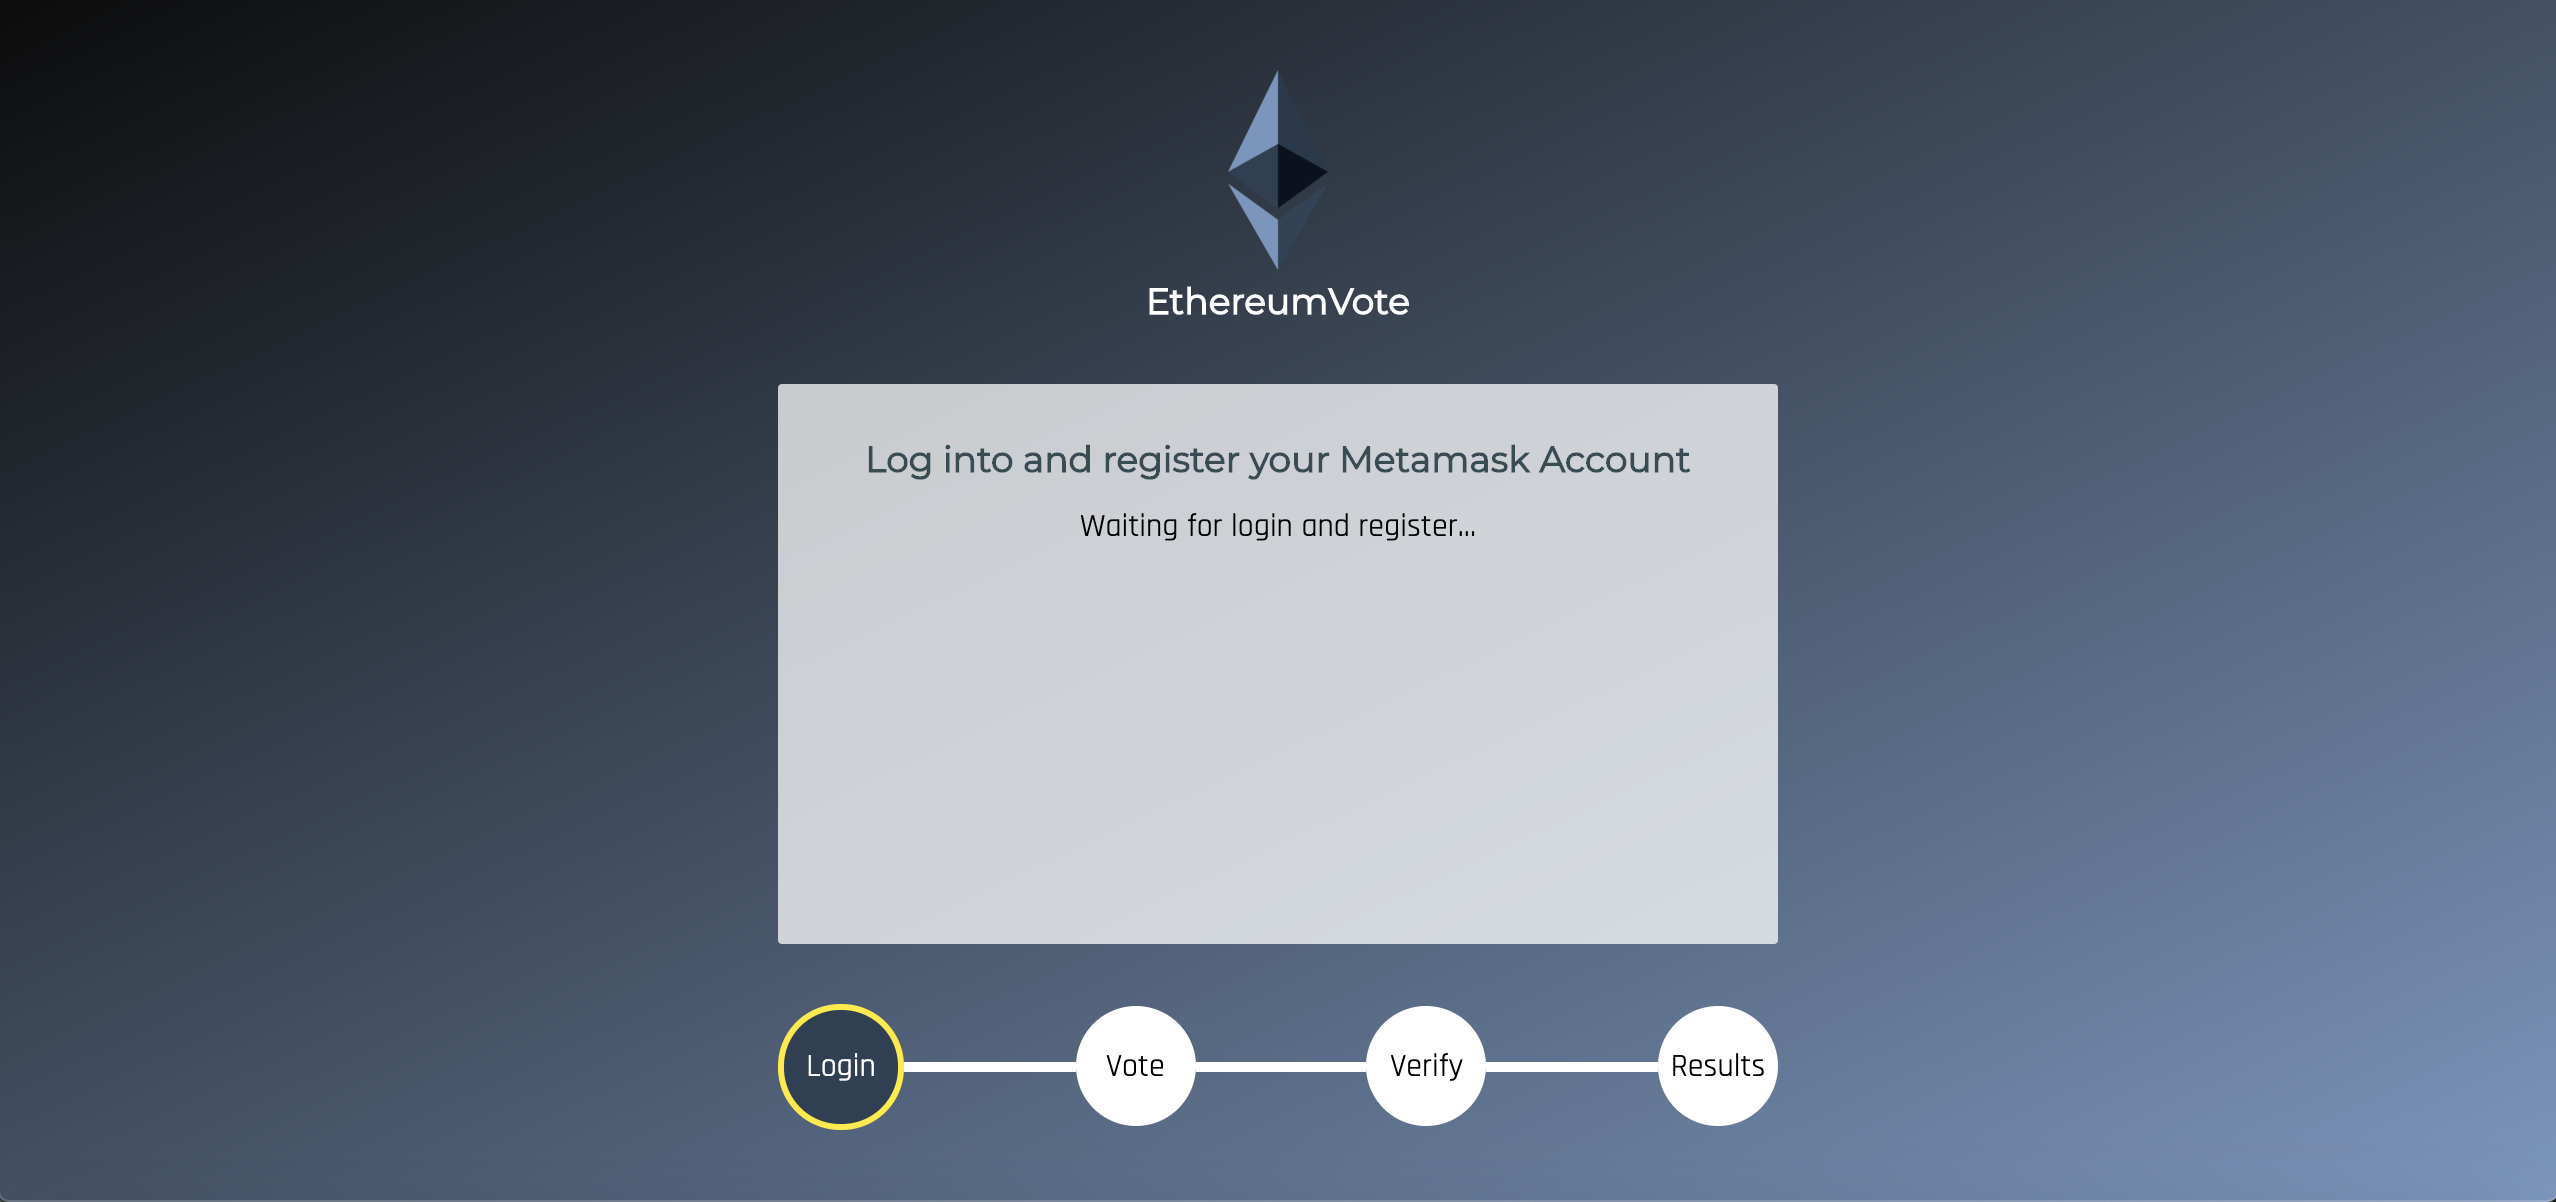
\includegraphics[width=\linewidth]{img/login.png}
		\caption{Het `login' scherm}
		\label{fig:login}
	\end{figure}
	\begin{figure}[h!]
		\centering
		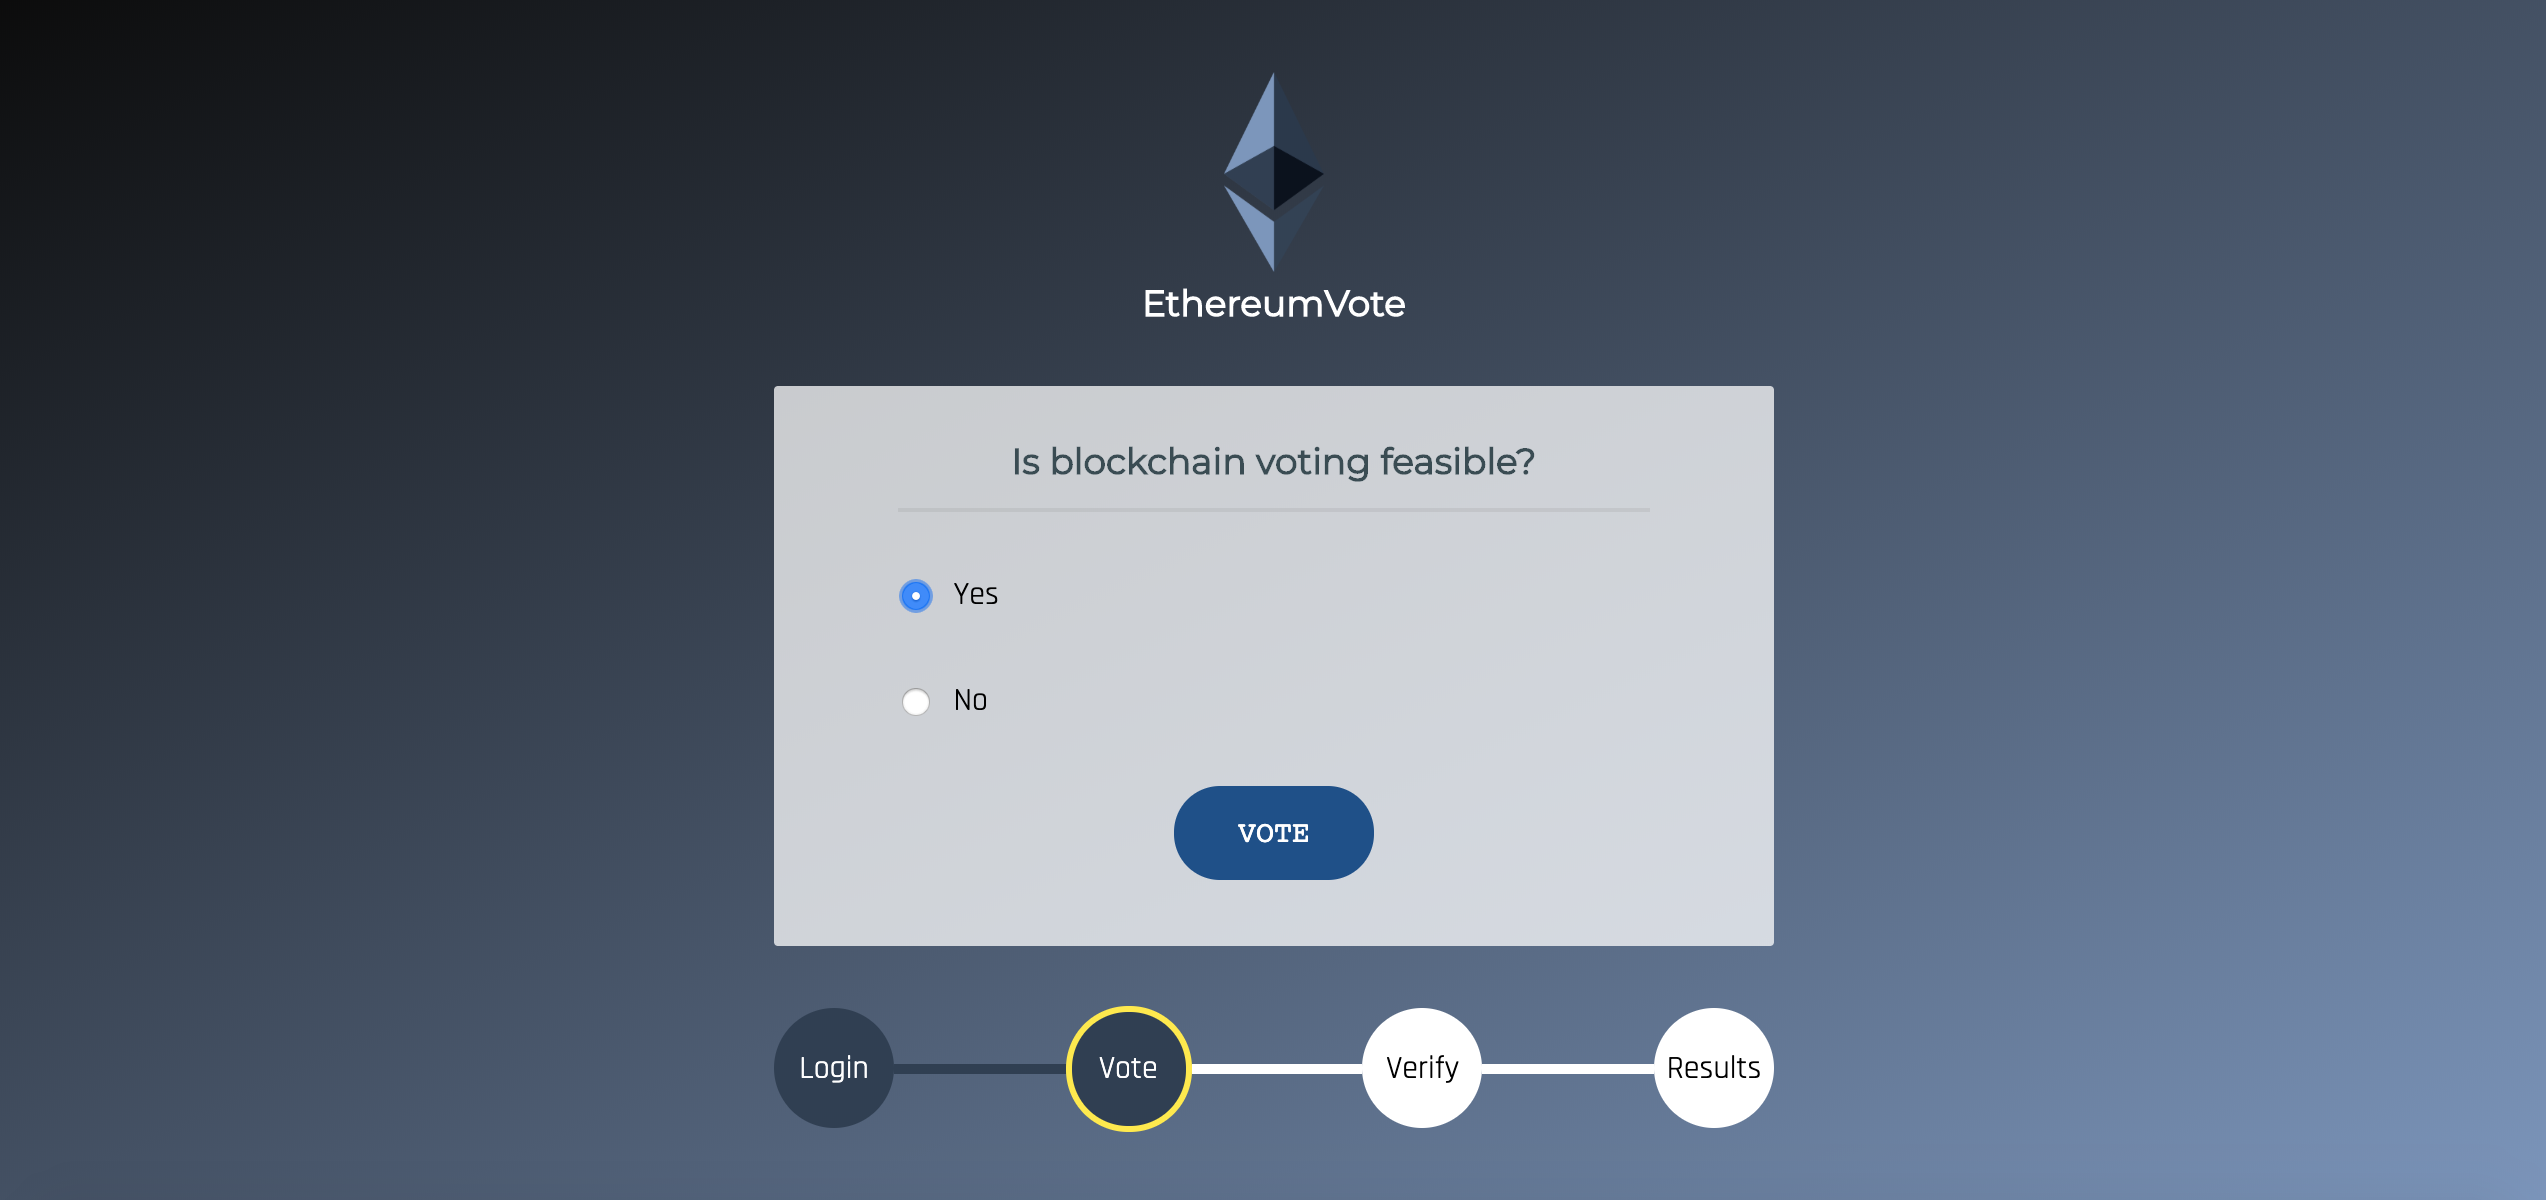
\includegraphics[width=\linewidth]{img/vote.png}
		\caption{Het `voting' scherm}
		\label{fig:vote}
	\end{figure}
	\begin{figure}[h!]
		\centering
		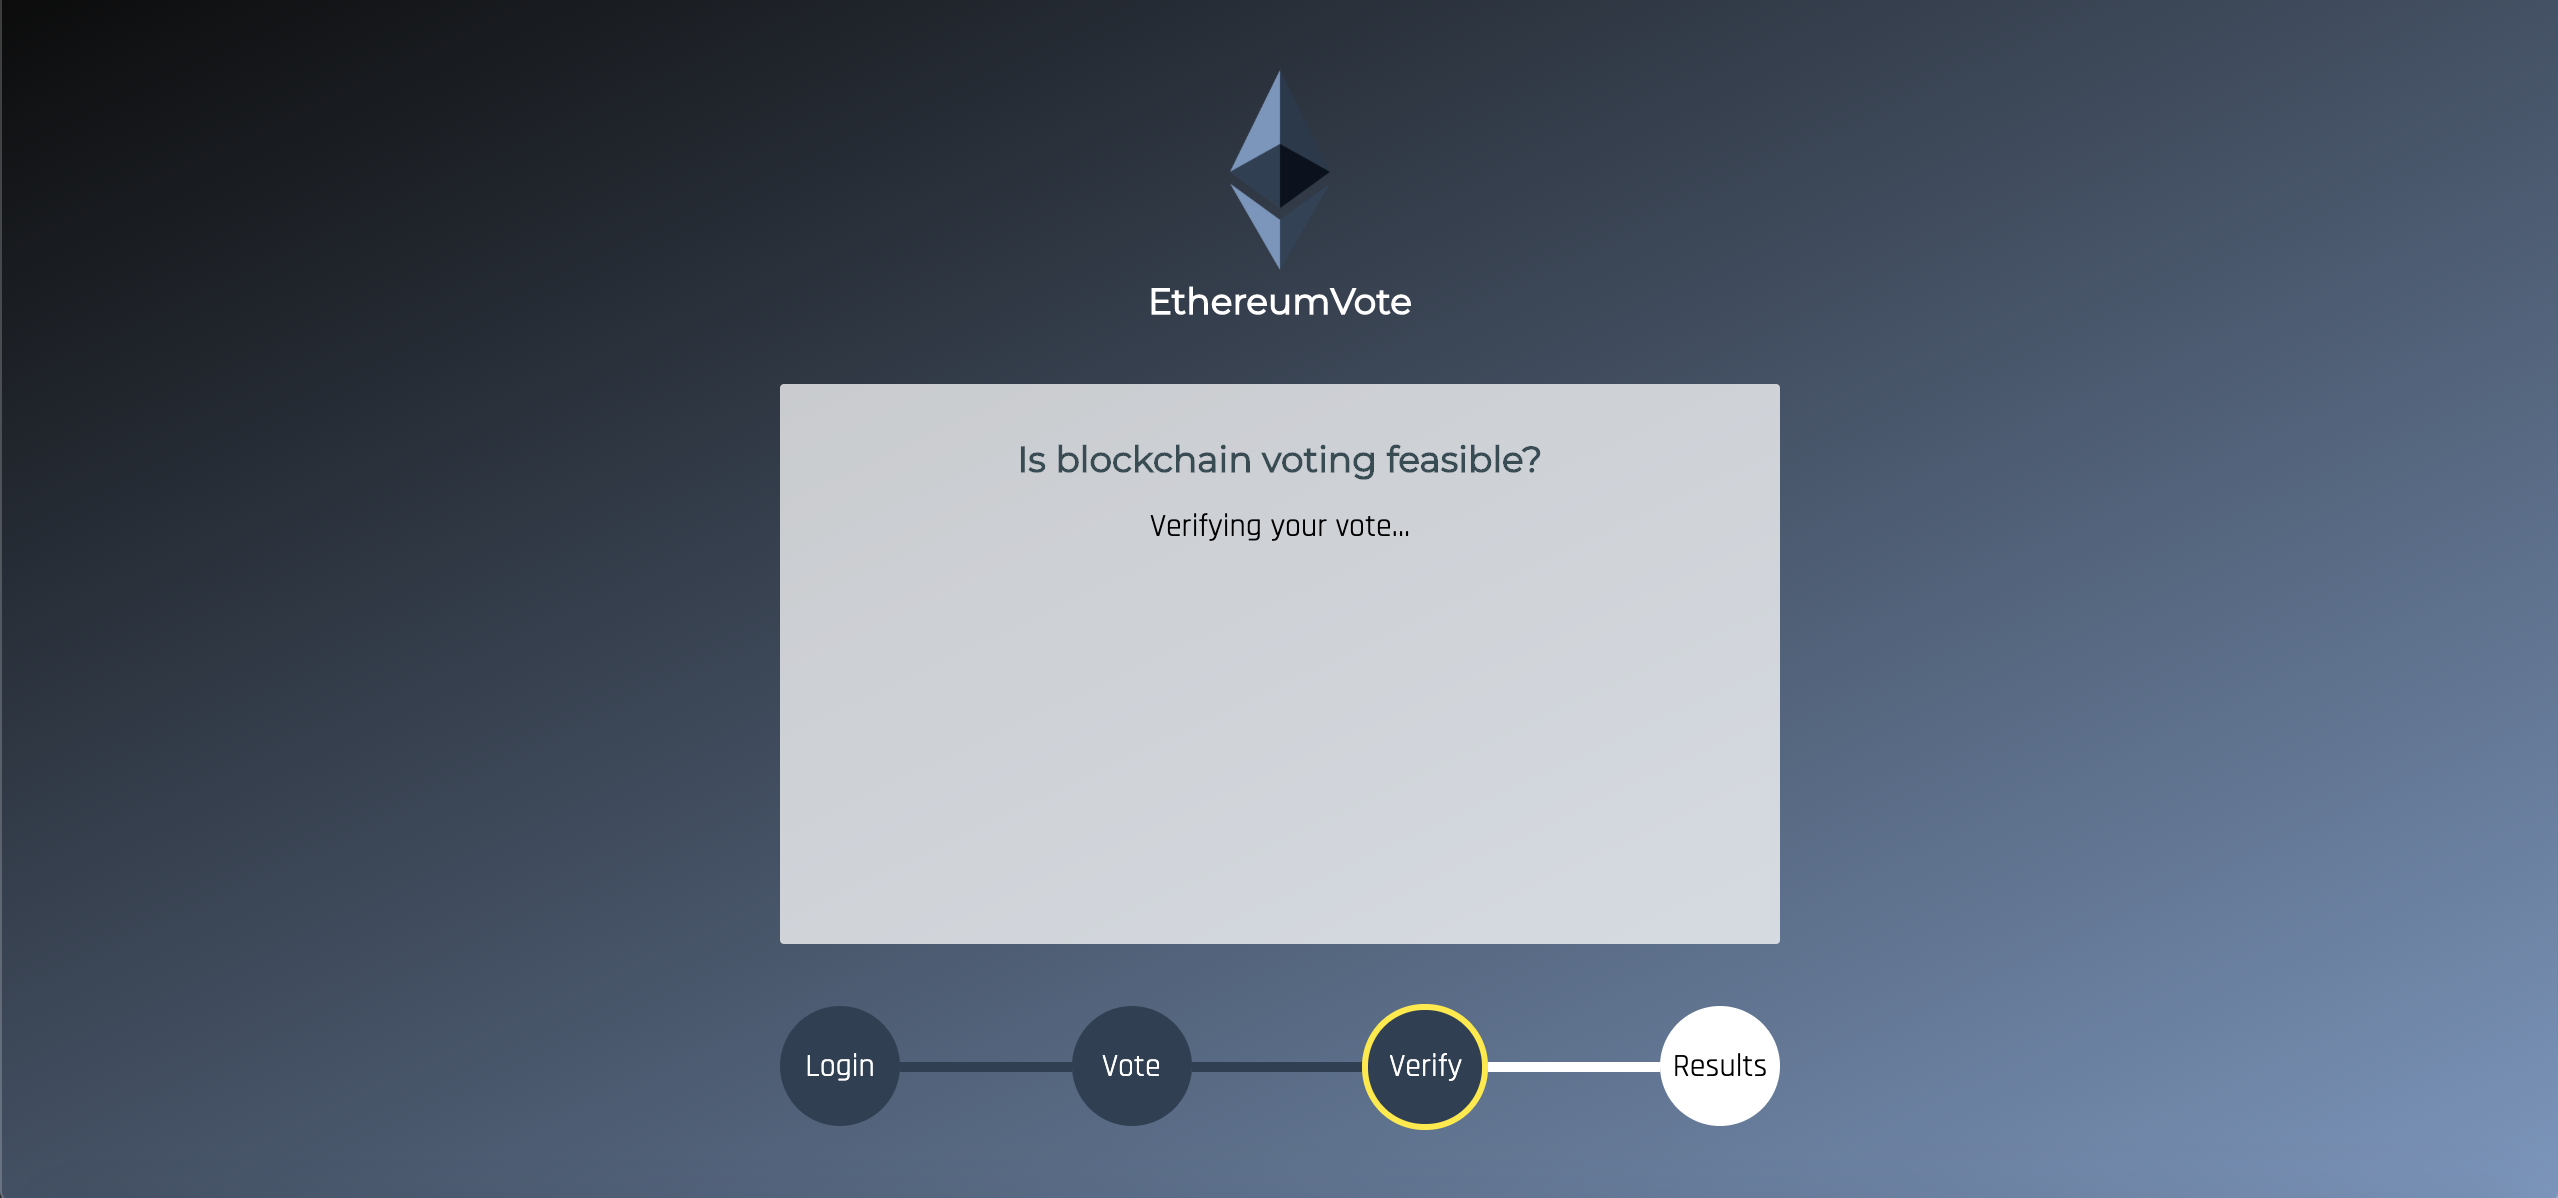
\includegraphics[width=\linewidth]{img/verify.png}
		\caption{Het `verify' scherm}
		\label{fig:verify}
	\end{figure}
	\begin{figure}[h!]
		\centering
		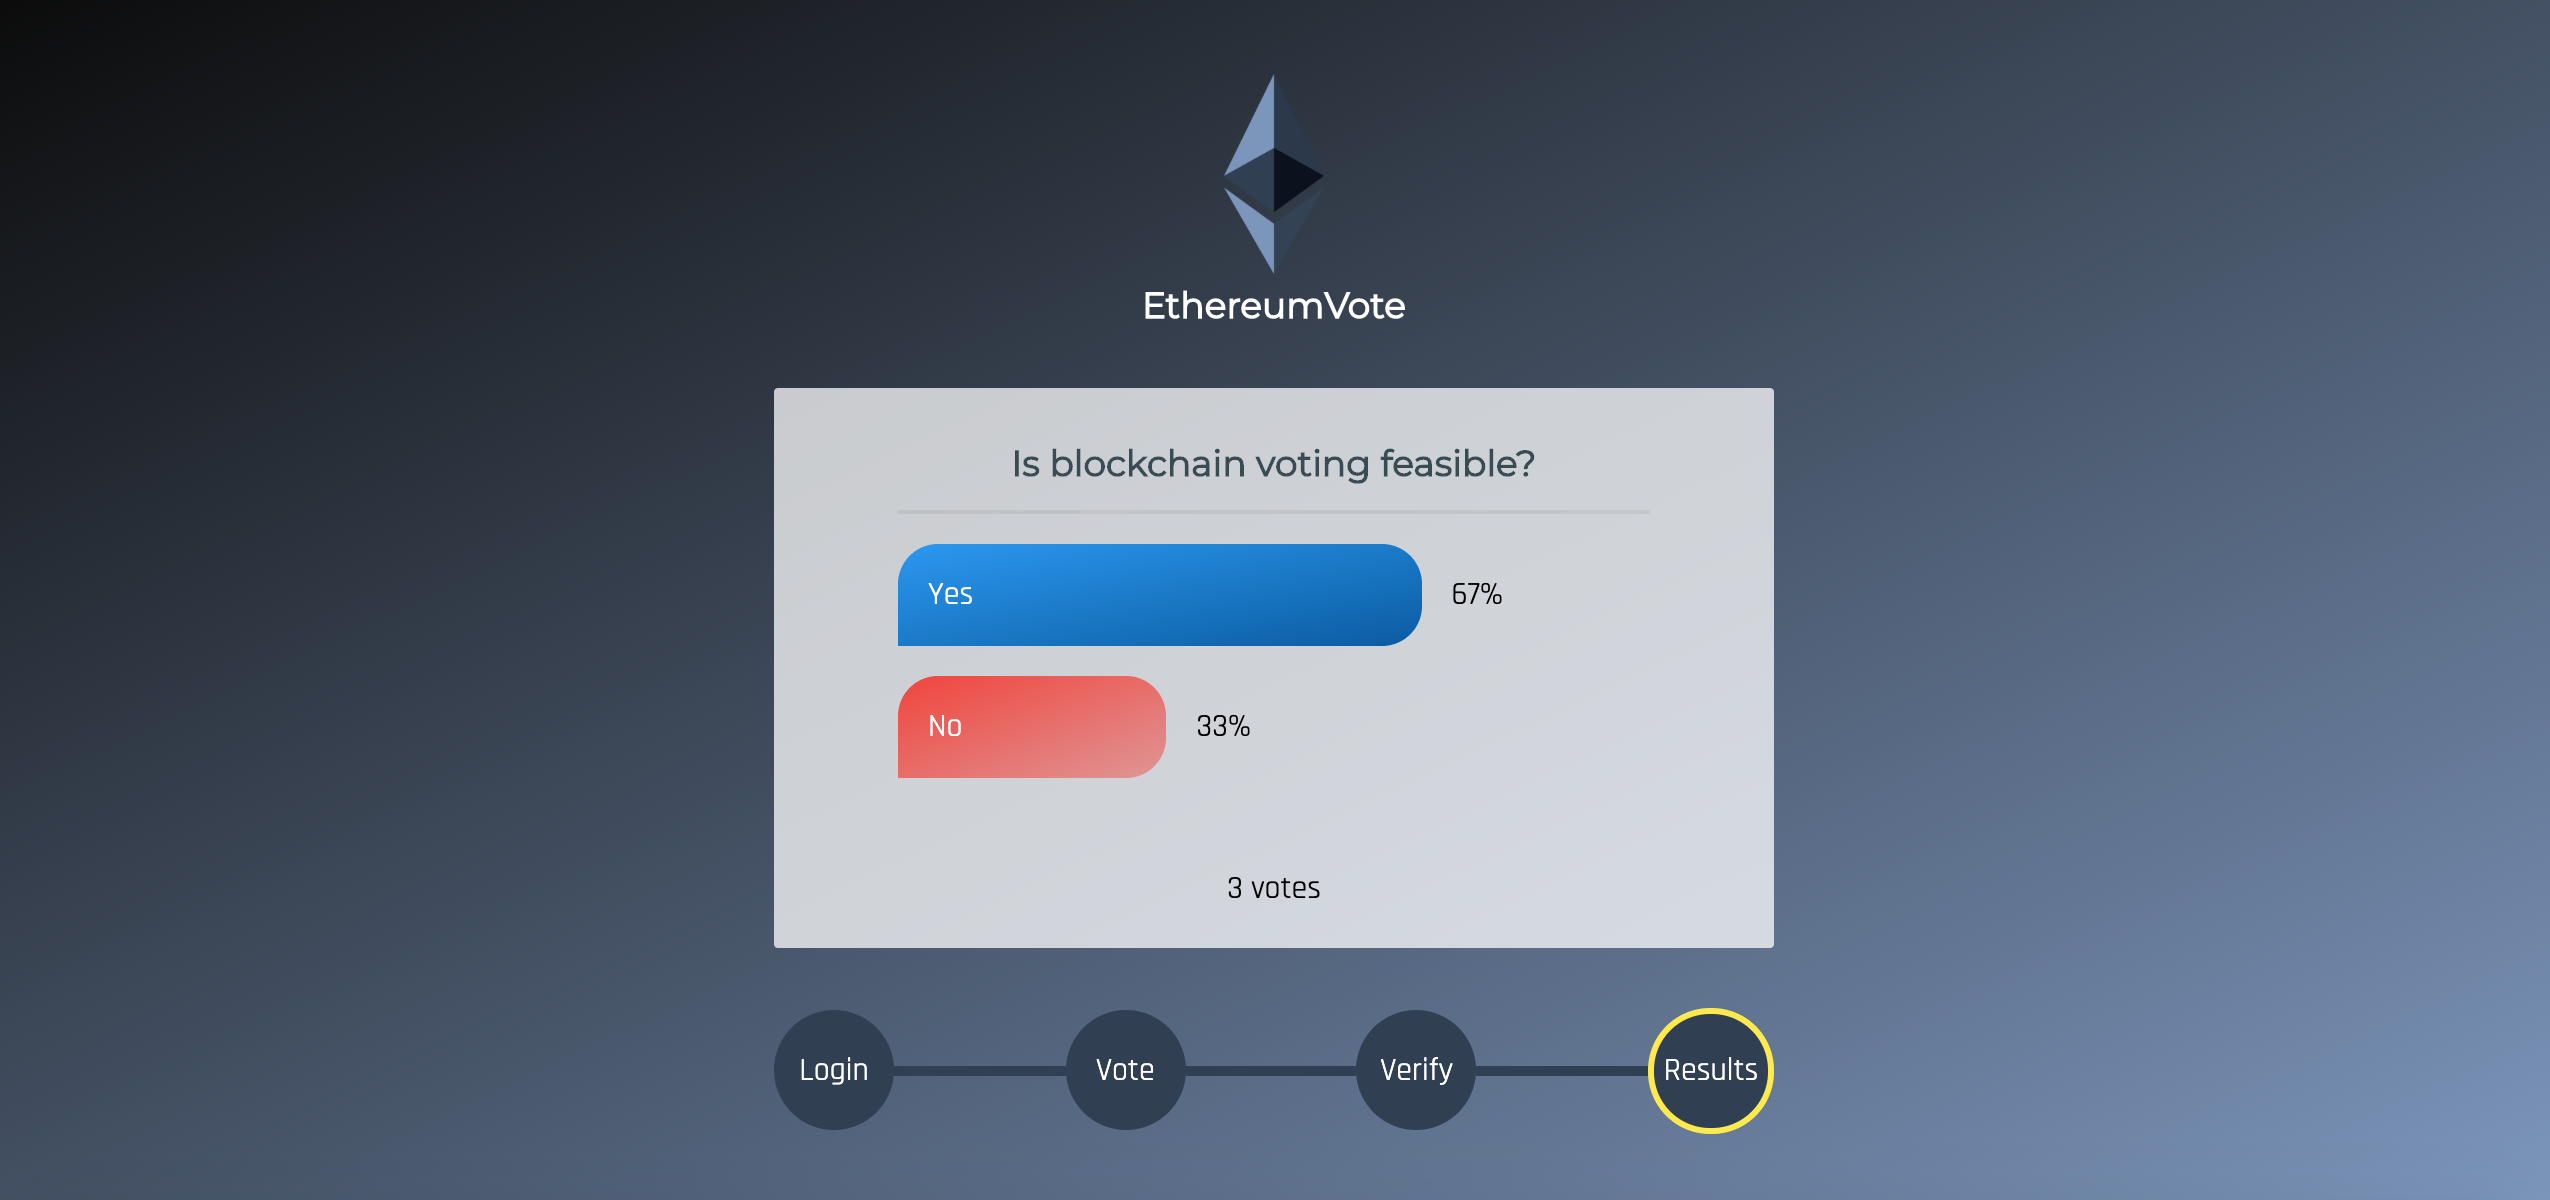
\includegraphics[width=\linewidth]{img/results.png}
		\caption{Het `results' scherm}
		\label{fig:results}
	\end{figure}
	\newpage
	\section{Eindresultaat}
	\subsection{Testen van Eindresultaat}
	Voordat we de werking van de volledige applicatie te testen, dienen we de onderstaande sequentiële stappen te ondernemen:
	\begin{enumerate}
		\item Opstarten van Ganache.
		\item Aanmaken van een nieuwe lokale blockchain-instantie in Ganache.
		\item Navigeren naar het back-end project in de console.
		\item Deployen van Smart contracts via console-commando \textit{truffle migrate} (eventueel \textit{- -reset}).
		\item Opstarten van Angular app .
		\item Inloggen op metamask.
		\item Importeren van accounts (geheime sleutels uit Ganache importeren in Metamask).
		\item Start manueel testen.
	\end{enumerate}
	Tenslotte kunnen we de applicatie testen als volgt:
	\begin{enumerate}
		\item Surfen naar de url waarop de app gehost wordt. (localhost:4200/ deployed instantie).
		\item Metamask: connecteren aan de blockchain via het ingelogde account.
		\item Metamask: `Register' transactie goedkeuren.
		\item DApp: stem uitbrengen op het stemscherm.
		\item Metamask: `Vote' transactie goedkeuren.
		\item DApp: resultaten van de verkiezing bekijken.
	\end{enumerate}
	Figuren \ref{fig:screen_login1}, \ref{fig:screen_login2}, \ref{fig:screen_voting1}, \ref{fig:screen_voting2}  en \ref{fig:screen_voting3} geven de verschillende stappen van het stemproces via de EthereumVoting app weer. Merk op: alle interacties met de blockchain worden direct geïnitialiseerd door de gebruiker vanuit de browser, maar moeten vervolgens ook nog eens bevestigd worden via de Metamask-plugin. De interacties gebeuren dus allemaal via een ingelogde Ethereum-wallet, wat het systeem volledig secuur maakt.
	\begin{figure}
		\centering
		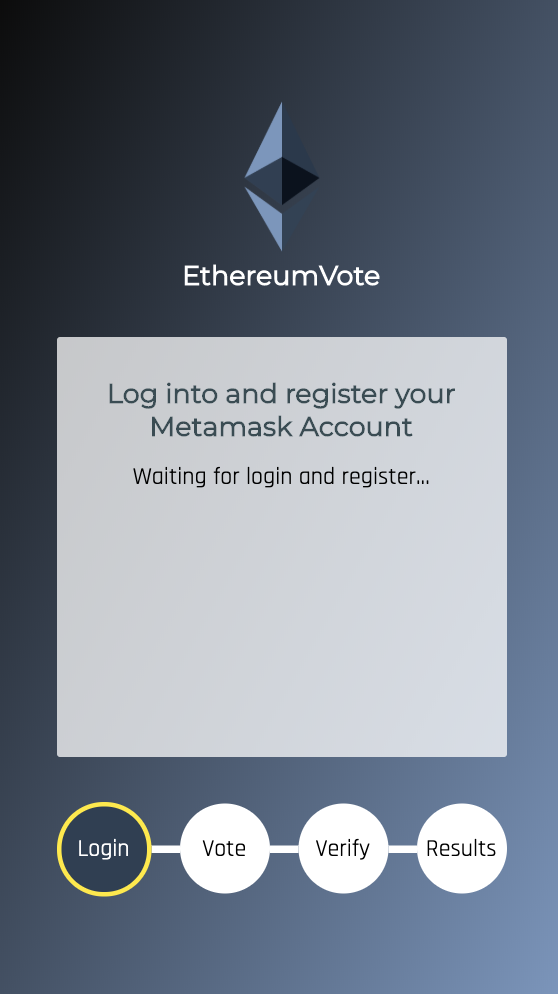
\includegraphics[width=\linewidth/3]{img/screen_login.png}
		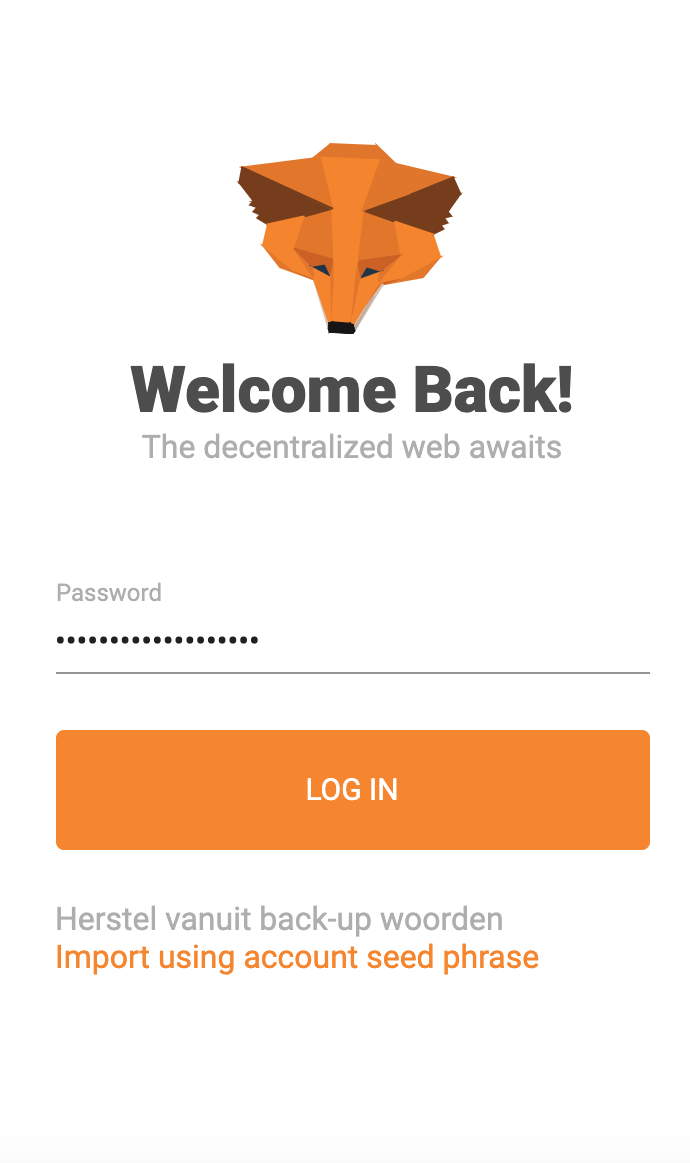
\includegraphics[width=\linewidth/3]{img/screen_metamask1.png}
		\caption{Inloggen op Metamask }
		\label{fig:screen_login1}
	\end{figure}
	\begin{figure}
		\centering
		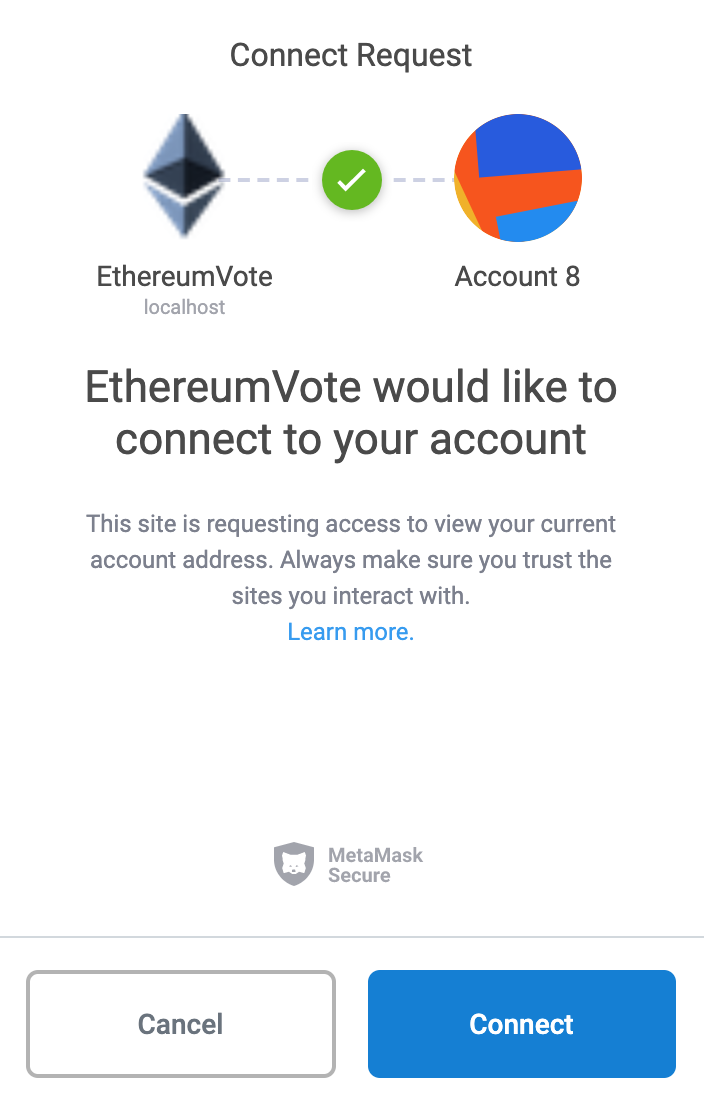
\includegraphics[width=\linewidth/3]{img/screen_metamask2.png}
		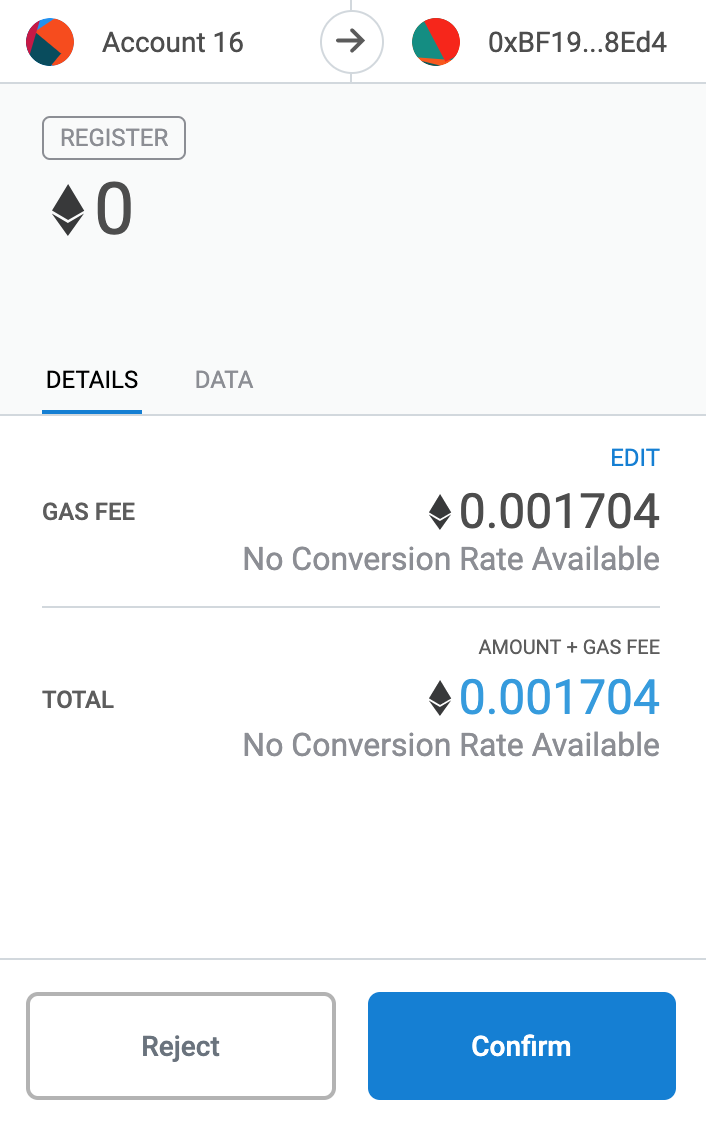
\includegraphics[width=\linewidth/3]{img/screen_metamask3.png}
		\caption{Verbinden met het Ethereum netwerk en registreren}
		\label{fig:screen_login2}
	\end{figure}
	\begin{figure}
		\centering
		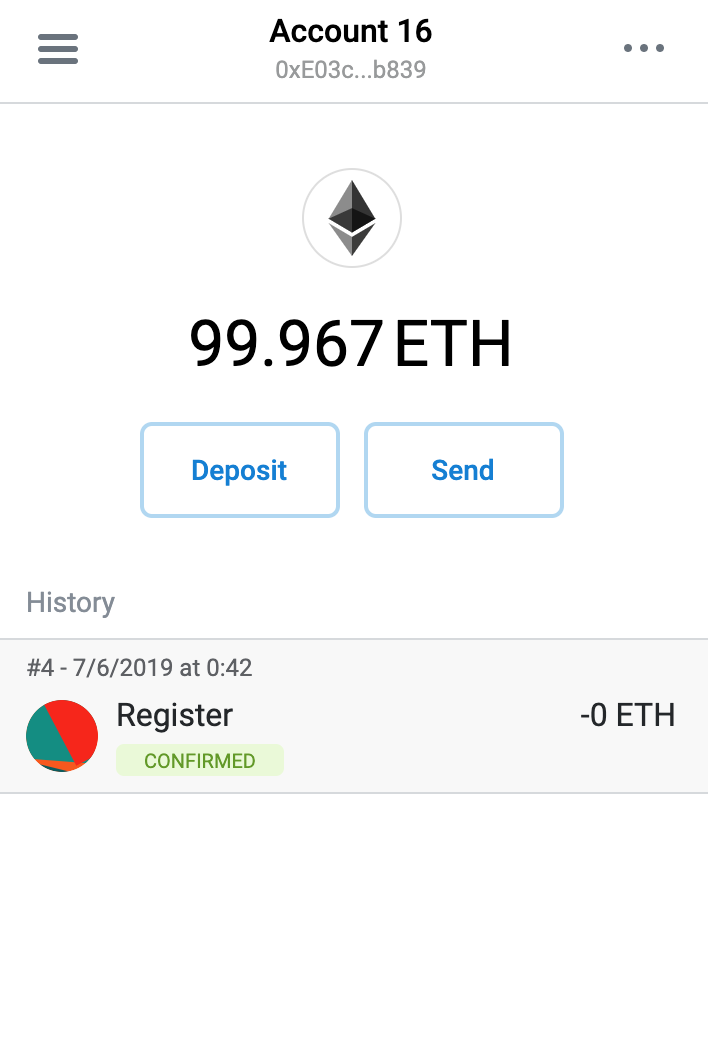
\includegraphics[width=\linewidth/3]{img/screen_metamask4.png}
		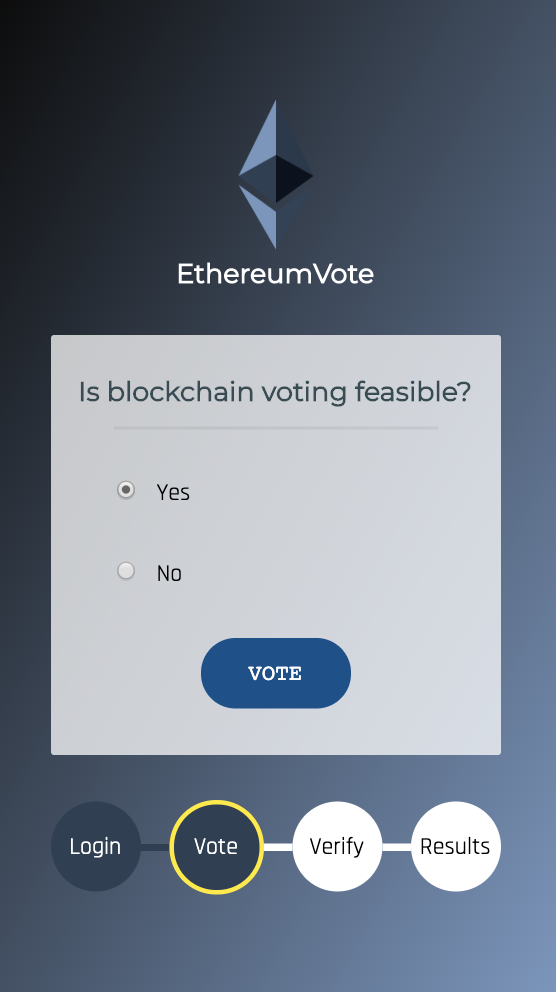
\includegraphics[width=\linewidth/3]{img/screen_voting.png}
		\caption{Stemmen, na de registratie-transactie voltooid is}
		\label{fig:screen_voting1}
	\end{figure}
	\begin{figure}
		\centering
		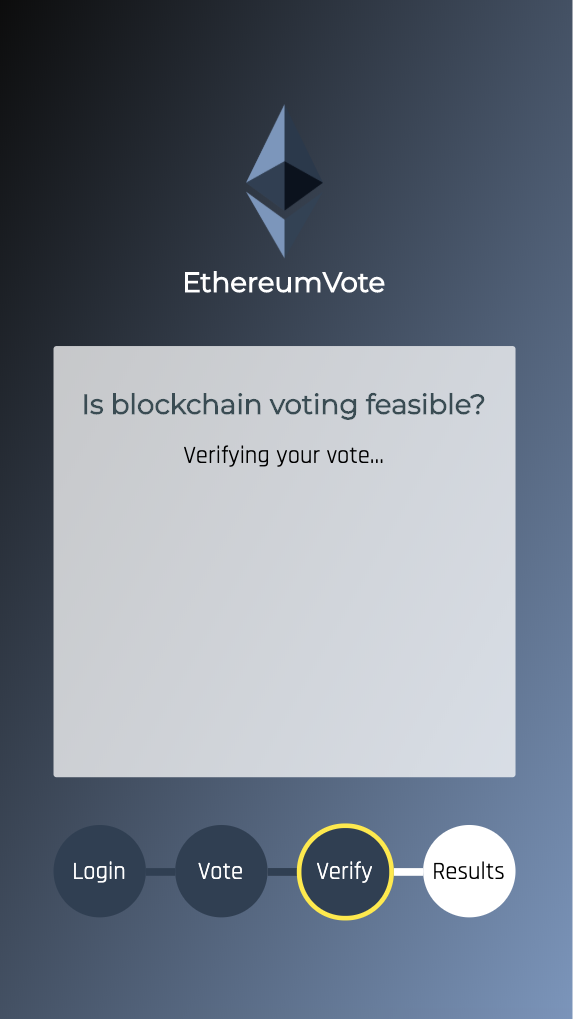
\includegraphics[width=\linewidth/3]{img/screen_verify.png}
		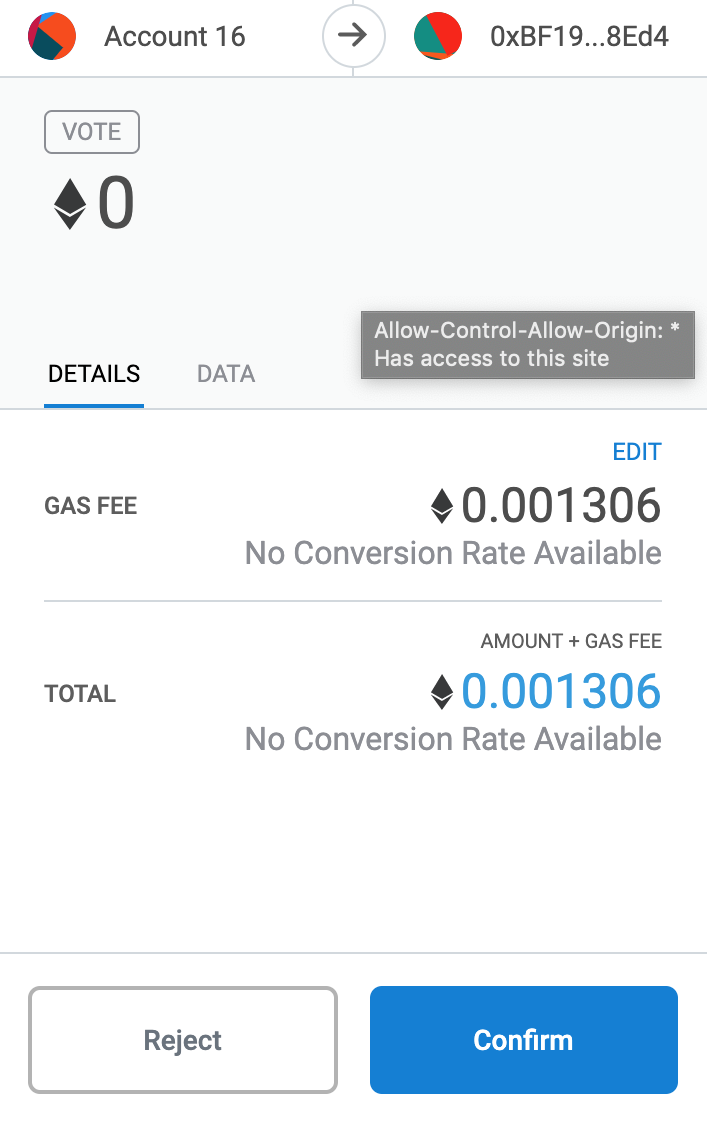
\includegraphics[width=\linewidth/3]{img/screen_metamask5.png}
		\caption{Stemtransactie goedkeuren en controleren}
		\label{fig:screen_voting2}
	\end{figure}
	\begin{figure}
		\centering
		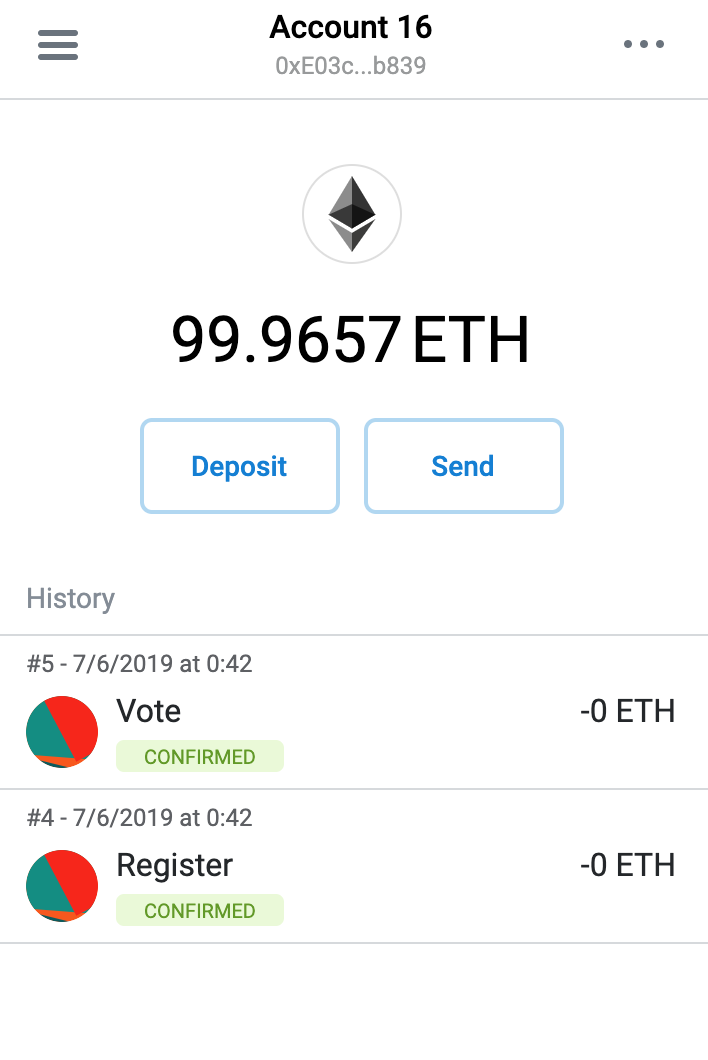
\includegraphics[width=\linewidth/3]{img/screen_metamask6.png}
		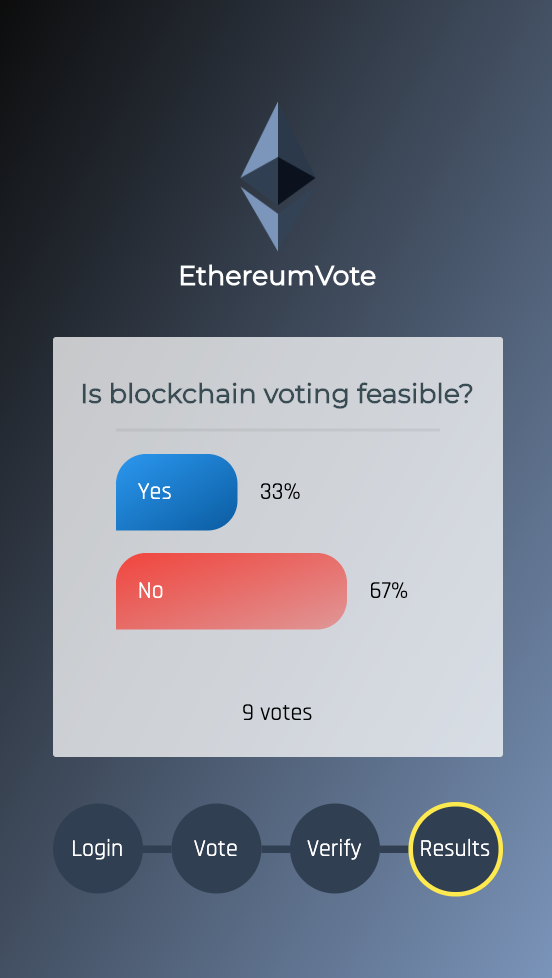
\includegraphics[width=\linewidth/3]{img/screen_results.png}
		\caption{De verkiezingsresultaten, na de stem-transactie voltooid is}
		\label{fig:screen_voting3}
	\end{figure}

	Eenmaal de bovenstaande stappen zijn doorlopen is deze handleiding ten einde gekomen: we hebben met succes een werkend \textbf{blockchain-gebaseerd stemsysteem} gebouwd op basis van Ethereum smart contracts, en deze gedeployed op een lokale blockchain. De werking van de smart contracts hebben we uitvoerig getest, via test files en de Truffle-console. Vervolgens hebben we onze smart contracts verbonden aan een webapplicatie gebouwd met het Angular javascript framework. De werking van de volledige DApp hebben we tenslotte in de browser bevestigd! 
	
	\subsection{Evaluatie Eindresultaat}
	Deze handleiding toont aan dat het ontwikkelen van een blockchain-gebaseerd stemsysteem eenvoudiger is dan ooit. De vele tools en hulpmiddelen waarvan we vandaag kunnen gebruik maken, zorgen voor lagen van abstractie en vereenvoudiging, die van blockchain een ontwikkelomgeving maken zoals alle andere.

	 Het stemsysteem dat we via deze handleiding hebben bekomen, is simpel en efficiënt. Het project is geschreven volgens de laatste standaarden en kan bijgevolg op alle moderne Ethereum-(test)netwerken draaien. Het is een perfect systeem voor kleinschalige verkiezingsscenario's: zaken zoals burgerinitiatieven, buurtcomités of raden van bestuur. EthereumVote biedt een drastische vereenvoudiging voor de organisatie en gebruiksvriendelijkheid van verkiezingen: organisatoren kunnen met enkele clicks een nieuwe verkiezing opzetten, gebruikers kunnen met nog minder clicks hun stem uitbrengen.
	 
	 Voor grotere verkiezingsscenario's zoals gemeentelijke, provinciale of nationale verkiezingen, is EthereumVote minder geschikt. De aard van de blockchain-technologie werkt hier in zekere zin tegen. Iedere transactie, elke interactie tussen gebruiker en systeem is immers publiek zichtbaar. In veel verkiezingen is volledige anonimiteit echter noodzakelijk. Om volledige anonimiteit op een blockchain te bereiken, moet men dus een manier vinden om geheimen te bewaren in een systeem waar alles wat opgeslagen wordt openbaar is. Er zijn systemen - zoals het OVNP (McCorry e.a., 2017) - die er in slagen dit te bereiken. Dergelijke oplossingen steunen echter op complexe cryptografie en zijn bijgevolg zeer inefficiënt en vaak te duur om in de context van een blockchain-netwerk te draaien.
	
	In de plaats van cryptografie aan het project toe te voegen, stellen we met EthereumVote een alternatieve oplossing voor: we encrypteren niet, maar verzekeren dat de accounts die onze kiezers gebruiken strikt anoniem blijven. De identiteit (naam, voornaam, leeftijd of geboortedatum) van de kiezer mag nooit worden gelinkt aan het adres van zijn of haar account. We garanderen dit door zelf de accounts te distribueren vòòr de verkiezing van start gaat. De accounts worden op random wijze toegewezen aan de in aanmerking komende kiezers. De accounts zijn daarvoor reeds bekend gemaakt aan het smart contract in de vorm van een \textit{whitelist}: enkel en alleen de accounts die door het smart contract gekend zijn mogen aan de verkiezingen deelnemen. 
	
	Het uitdelen/verkopen van de accounts is in dit geval wel iets wat een bepaalde vorm van \textit{centrale autoriteit} vergt. De organisator van de verkiezing krijgt in zekere zin ook extra macht: deze persoon of groep van personen kan via het account immers bepalen wie er zal deelnemen aan de verkiezing. Deze  twee nadelen zijn echter aanvaardbaar, bovendien worden ze teniet gedaan door de reeds genoemde voordelen van EthereumVote.
	
	

	

	
	
	
	
	
	
	
	
	
	
	
	
	
	
	
	
	
	
	
	
	

	








